\documentclass{article}

\usepackage{epsfig}
\usepackage[mathscr]{eucal}
\usepackage{amsfonts}
\usepackage{amscd}
\usepackage{amsmath}
\usepackage{array}
\usepackage{amssymb}
%\usepackage[backend=bibtex8, sorting=none]{biblatex}
\usepackage{colordvi}
\usepackage{enumerate}
\usepackage{graphicx}
\usepackage{booktabs}
\usepackage[footnotesize]{caption}
\usepackage{fancyhdr}
\usepackage{pdfpages}
\usepackage{slashed}
\usepackage{tabularx}
\usepackage{longtable}
\usepackage{array}
\usepackage{caption}
\usepackage{subcaption}

%\usepackage{relsize}
\usepackage{color}
\usepackage{rotating}

\usepackage{slashed}

\usepackage{epsfig,amsmath,graphicx,amssymb,listings,slashed}
\usepackage[colorlinks,citecolor=blue,urlcolor=blue,linkcolor=blue]{hyperref}
\usepackage[outercaption]{sidecap}

\usepackage{booktabs}

%\smartqed
%\usepackage[T1]{fontenc}
\usepackage[utf8]{inputenc}

\usepackage{epsfig,amsmath,graphicx,amssymb,listings,slashed}
\usepackage[colorlinks,citecolor=blue,urlcolor=blue,linkcolor=blue]{hyperref}

\setlength{\evensidemargin}{0cm}
\setlength{\oddsidemargin}{0cm}
\setlength{\topmargin}{0.00cm}
\setlength{\textwidth}{16.0cm}
\setlength{\textheight}{24.00cm}
\setlength{\headheight}{0cm}
\setlength{\headsep}{0cm}
\setlength{\voffset}{0cm}
\setlength{\paperheight}{29cm}

\definecolor{ourbrown}{RGB}{155,100,15}
\definecolor{ourcyan}{RGB}{20,165,165}
\definecolor{ourpurple}{RGB}{145,0,140}
\definecolor{darkorange}{RGB}{225,100,0}
\definecolor{darkgreen}{RGB}{0,170,0}
\definecolor{darkgray}{RGB}{80,80,80}

\setlength{\marginparwidth}{20mm}







\begin{document}

\title{ Machine Learning - SS 2021 \\ Exercise 3: Synthetic Data }


	\author{Federico Ambrogi, \textcolor{blue} {e1449911@student.tuwien.ac.at } \\
	Adam Höfler, \textcolor{blue} {e11847620@student.tuwien.ac.at } \\
	Matteo Panzeri \textcolor{blue}{12039996@student.tuwien.ac.at } \\
    TU Wien }


%\ead{federico.ambrogi@univie.ac.at}




\maketitle
\setcounter{tocdepth}{2}
\tableofcontents

\section*{Introduction}
In this document we describe the results of the implementation of synthesizing algorithms to create synthetic replicas of three different data sets. We test them for their ability to create replicas of the original data set.



\section{Data Sets Description}
Here we briefly introduce our datasets, analyze the distributions of the input data and check for significant correlations between variables.

\clearpage
\subsection{Income Data Set}
The data set \cite{income} provides us information about people, like: age, workclass, education, marital-status, occupation, capital-gain, ecc...\\
Our purpose is to determine if a person income is lower or greater than a given value specifically the threshold is 50000 Dollars per year. The distribution of a selection of relevant features, as well as a scatter plot to highlight pair-wise correlations are shown in Fig. \ref{pairplot_income}, while a more general view on the correlations including all features are shown in Fig. \ref{correlation_income}.\\


\begin{figure}[h!]
	\centering
	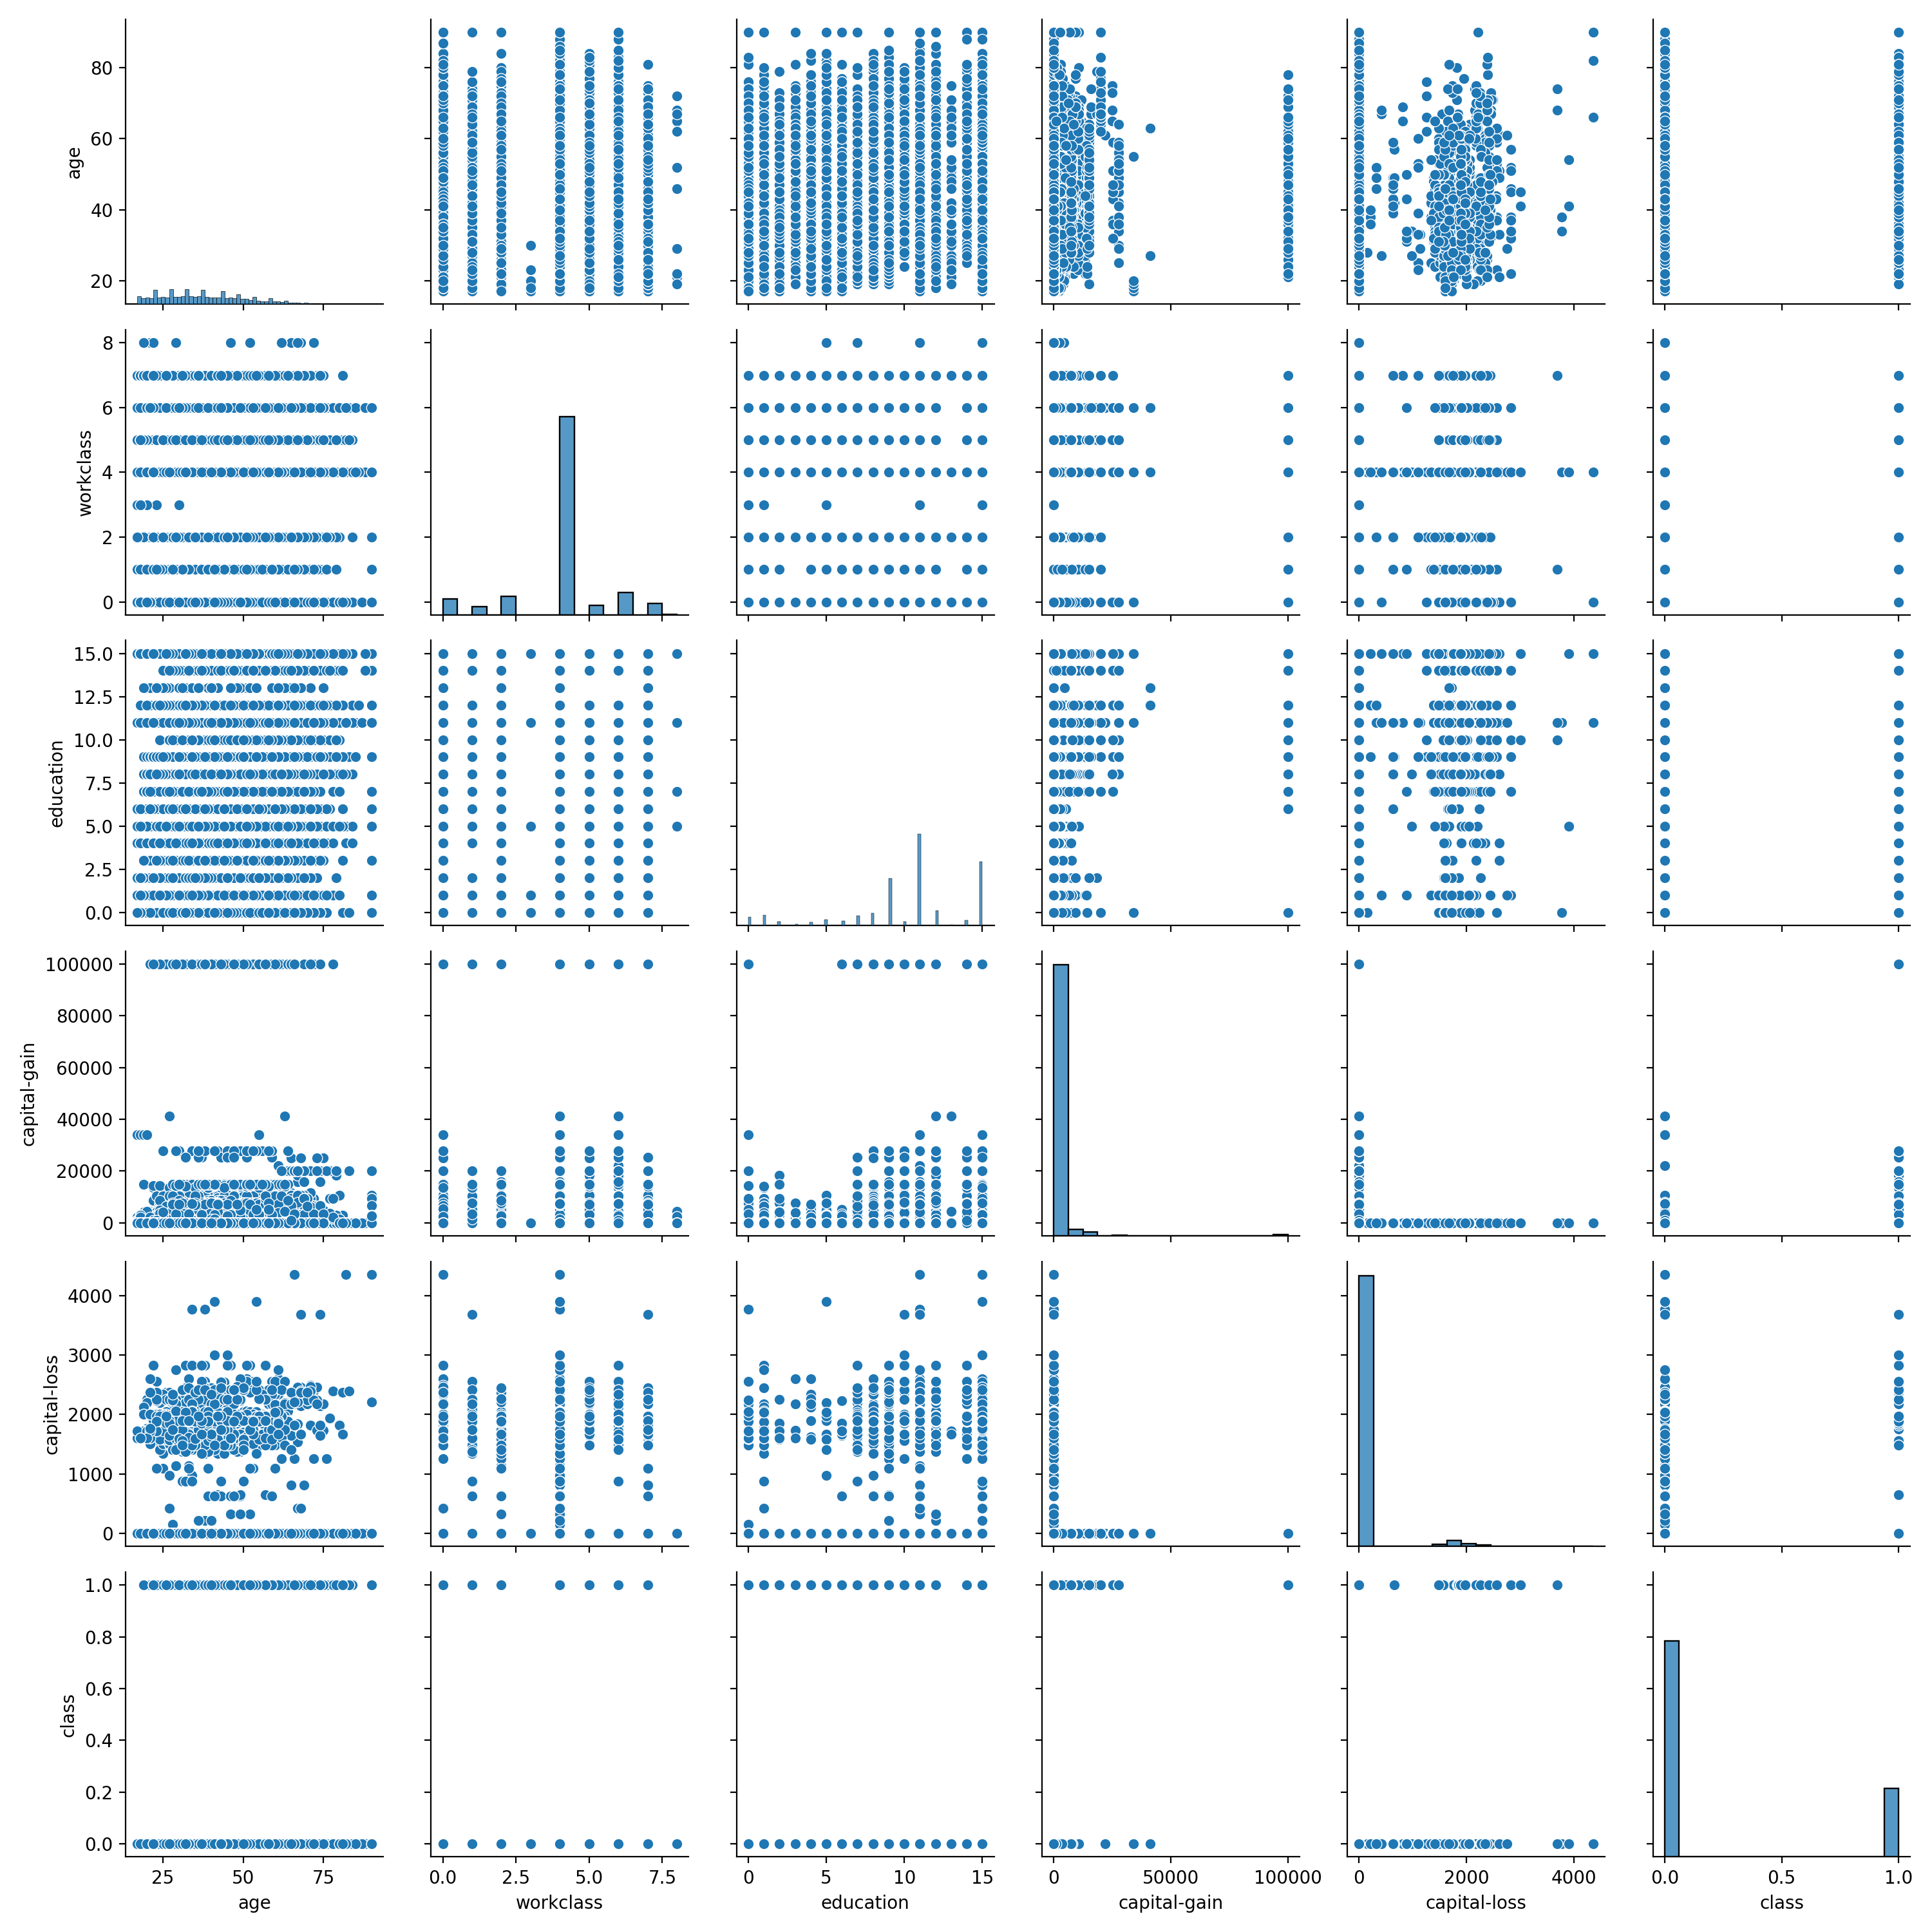
\includegraphics[width=0.8\textwidth]{../plots/income_pairplot_reduced_original.png}
	\caption{ Distributions and pair-wise correlation for the features of the "income" data set.}
	\label{pairplot_income}
\end{figure}


\begin{figure}[h!]
	\centering
	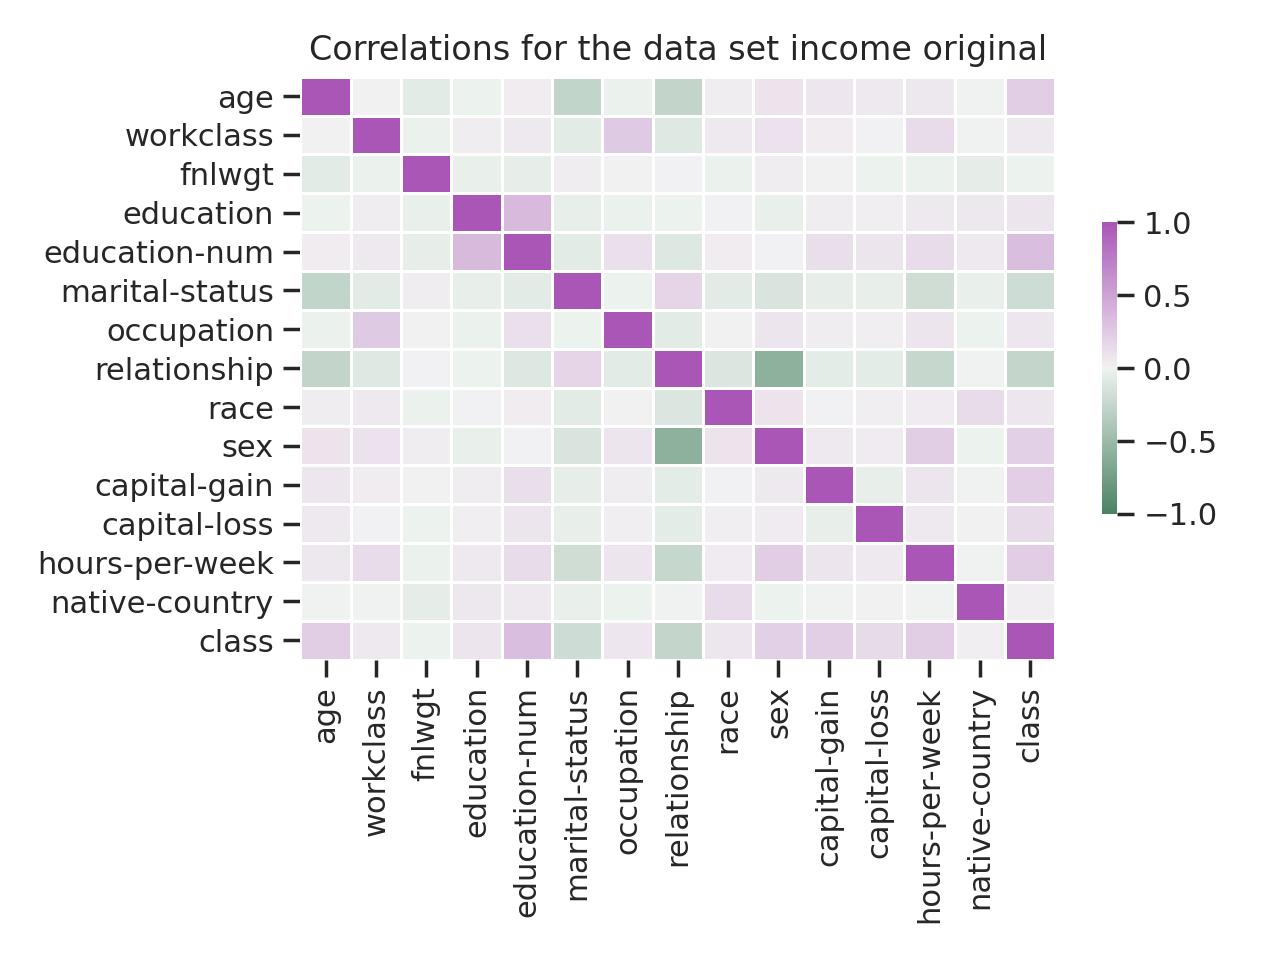
\includegraphics[width=0.5\textwidth]{../plots/income_correlations_original.png}
	\caption{Correlation matrix for the "income" data set. }
	\label{correlation_income}
\end{figure}



\clearpage
\subsection{Titanic Data Set}
The Titanic data set \cite{titanic} contains informations about the Titanic's passengers. Given the observations we want to determine if a given person, represented by an observation, will survive on the Titanic.\\
Some features of the dataset are: Name, sex, age, Passenger class, ticket fare, where the passenger embarked, etc.

\begin{figure}[h!]
	\centering
	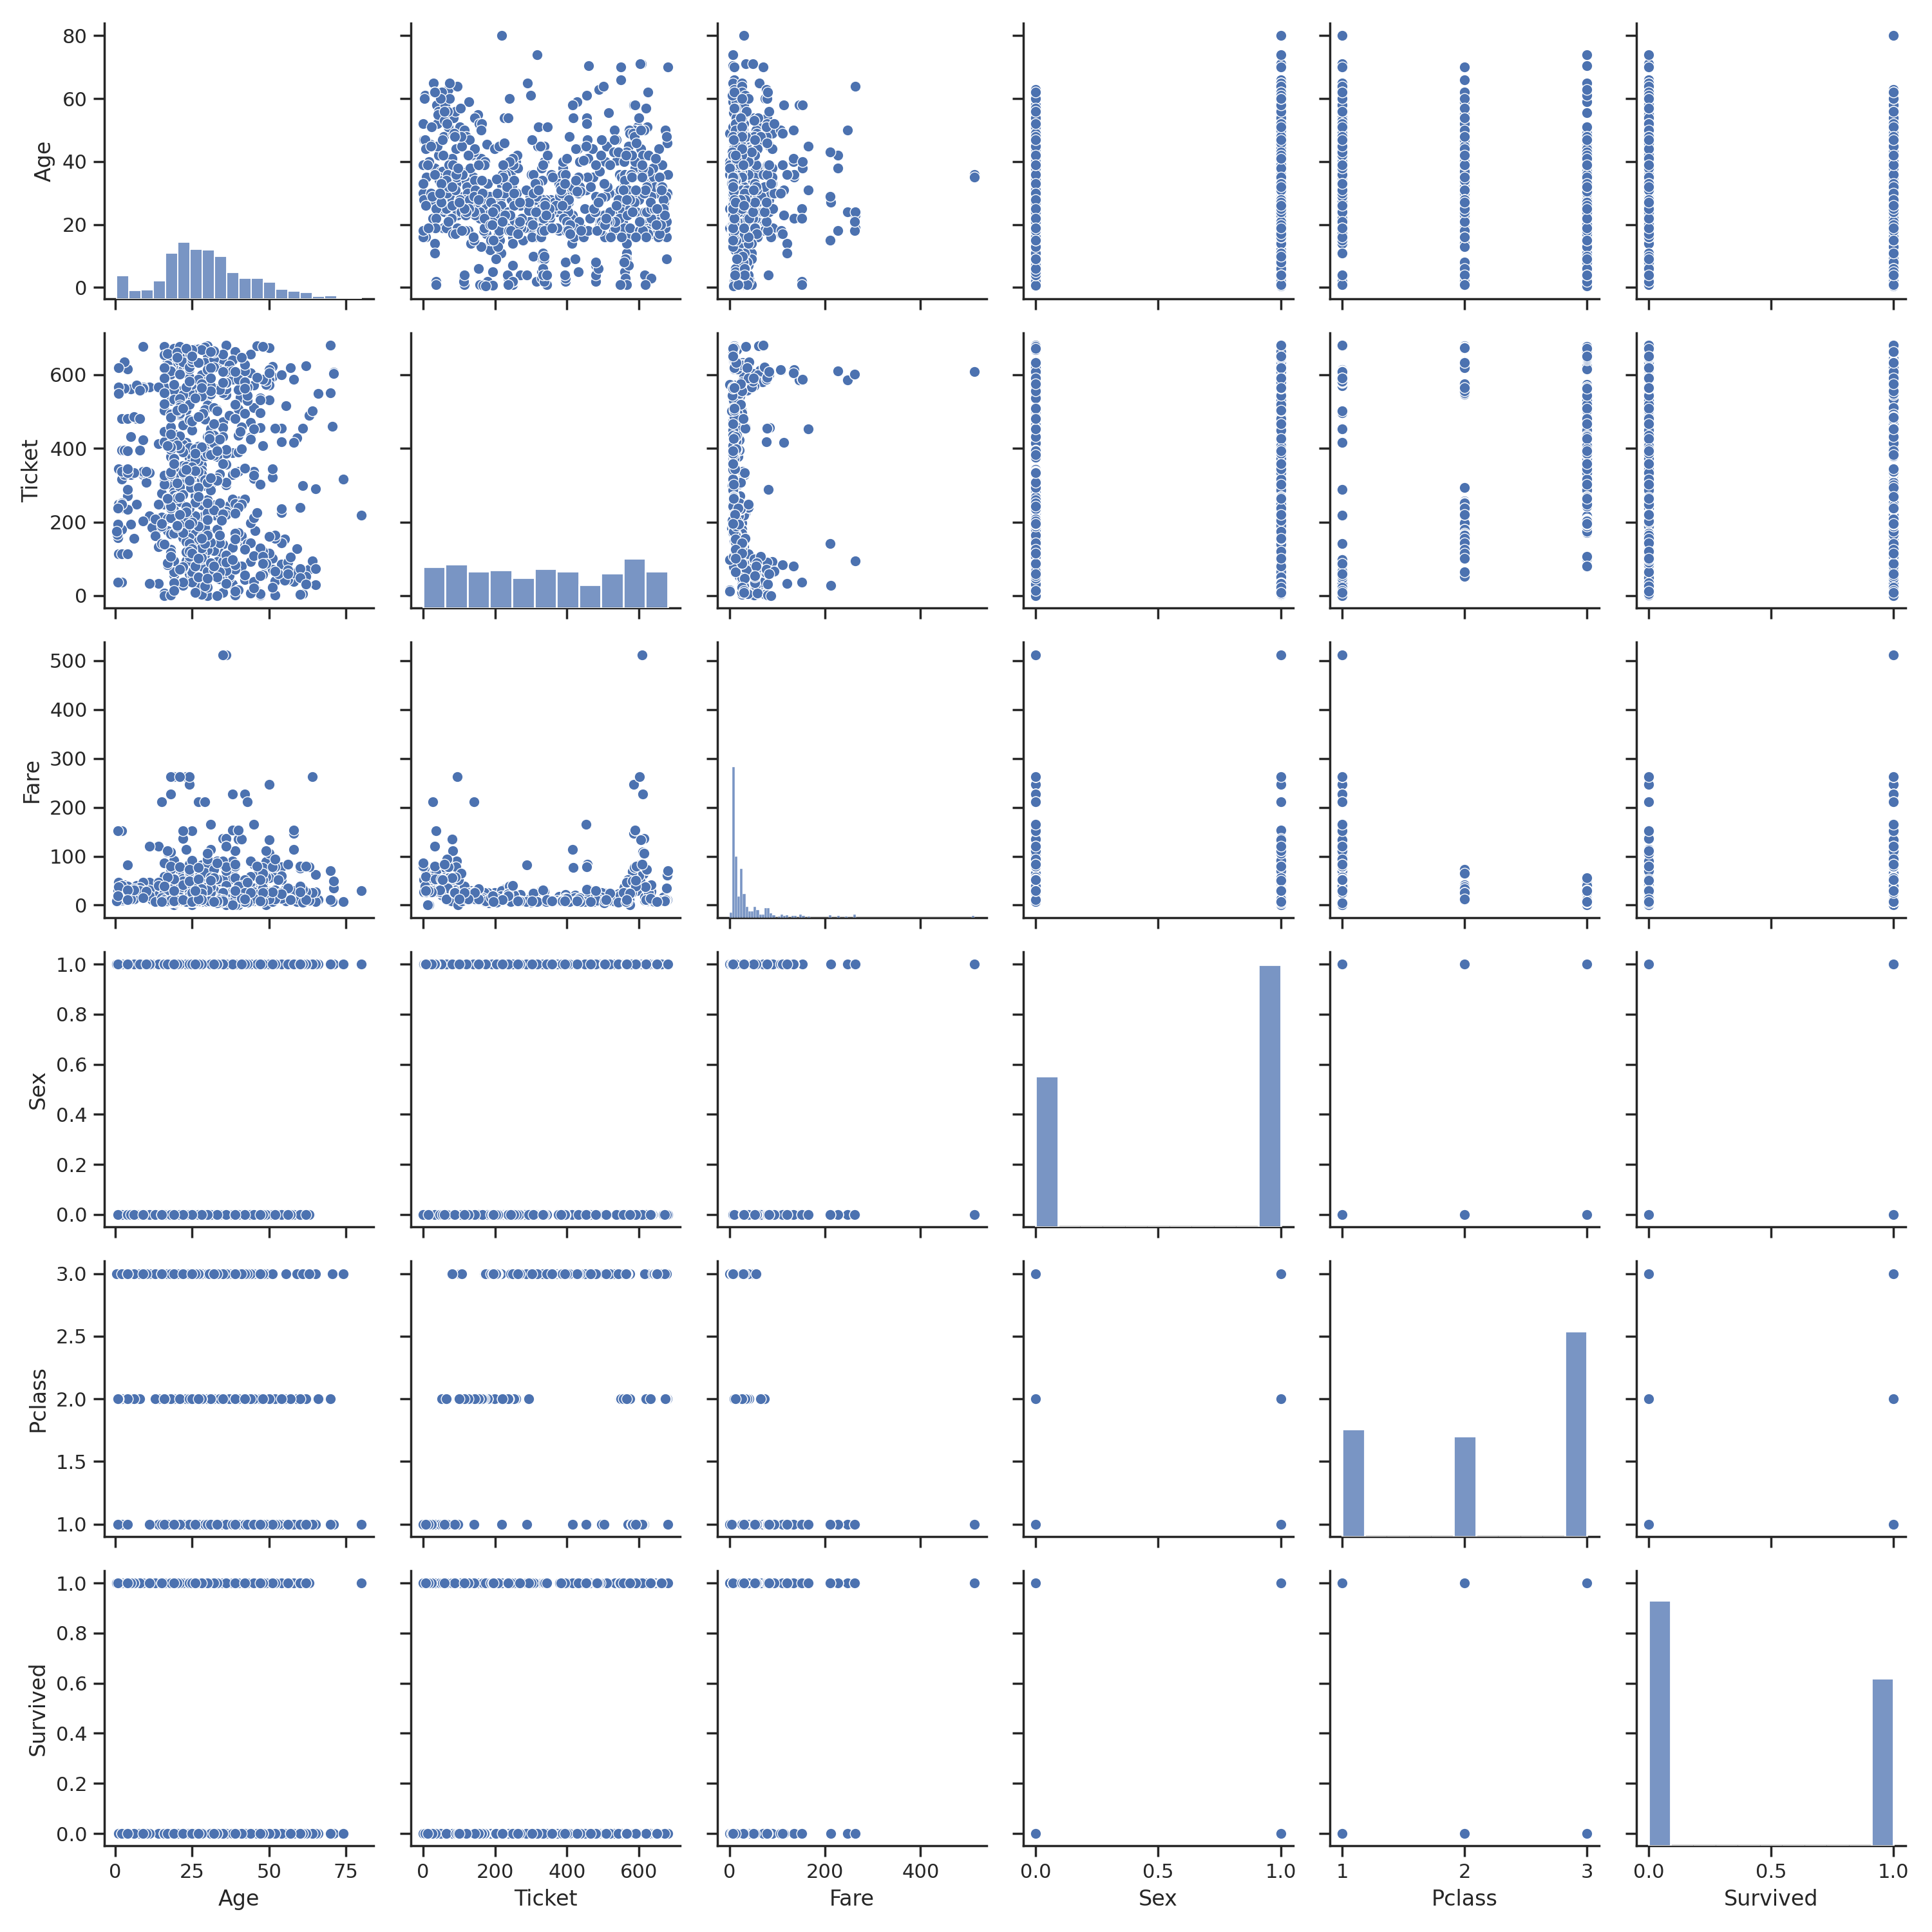
\includegraphics[width=0.8\textwidth]{../plots/titanic_pairplot_reduced_original.png}
	\caption{ Distributions and pair-wise correlation for the features of the "social" data set.}
	\label{pairplot_income}
\end{figure}


\begin{figure}[h!]
	\centering
	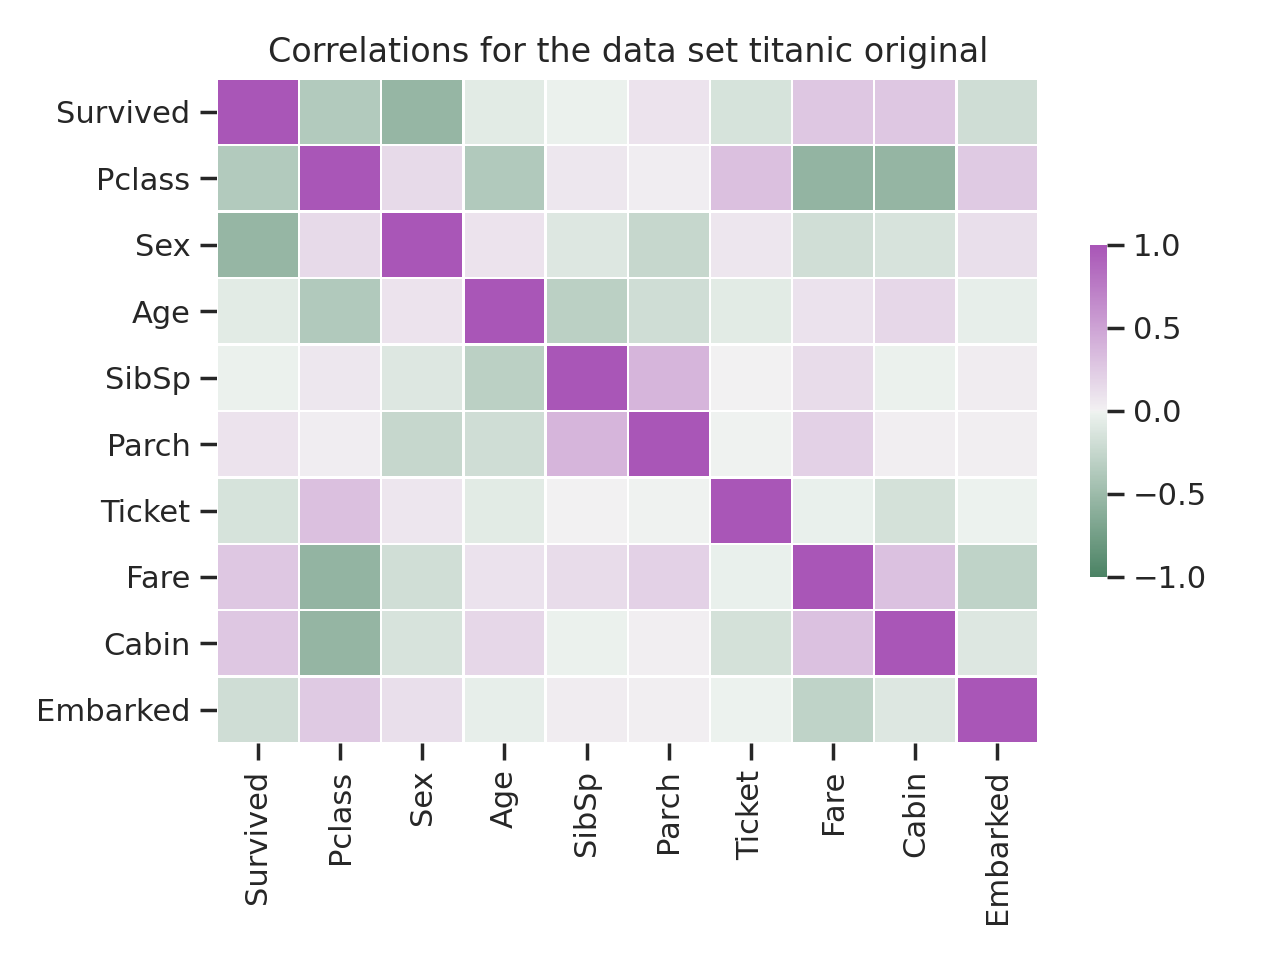
\includegraphics[width=0.5\textwidth]{../plots/titanic_correlations_original.png}
	\caption{Correlation matrix for the "social" data set. }
	\label{correlation_income}
\end{figure}


\clearpage
\subsection{Social Data Set}
The Social network ads data set \cite{social} collects information about social network users in particular age,sex and income. Our objective is to understand if an user will buy the advised good.

\begin{figure}[h!]
	\centering
	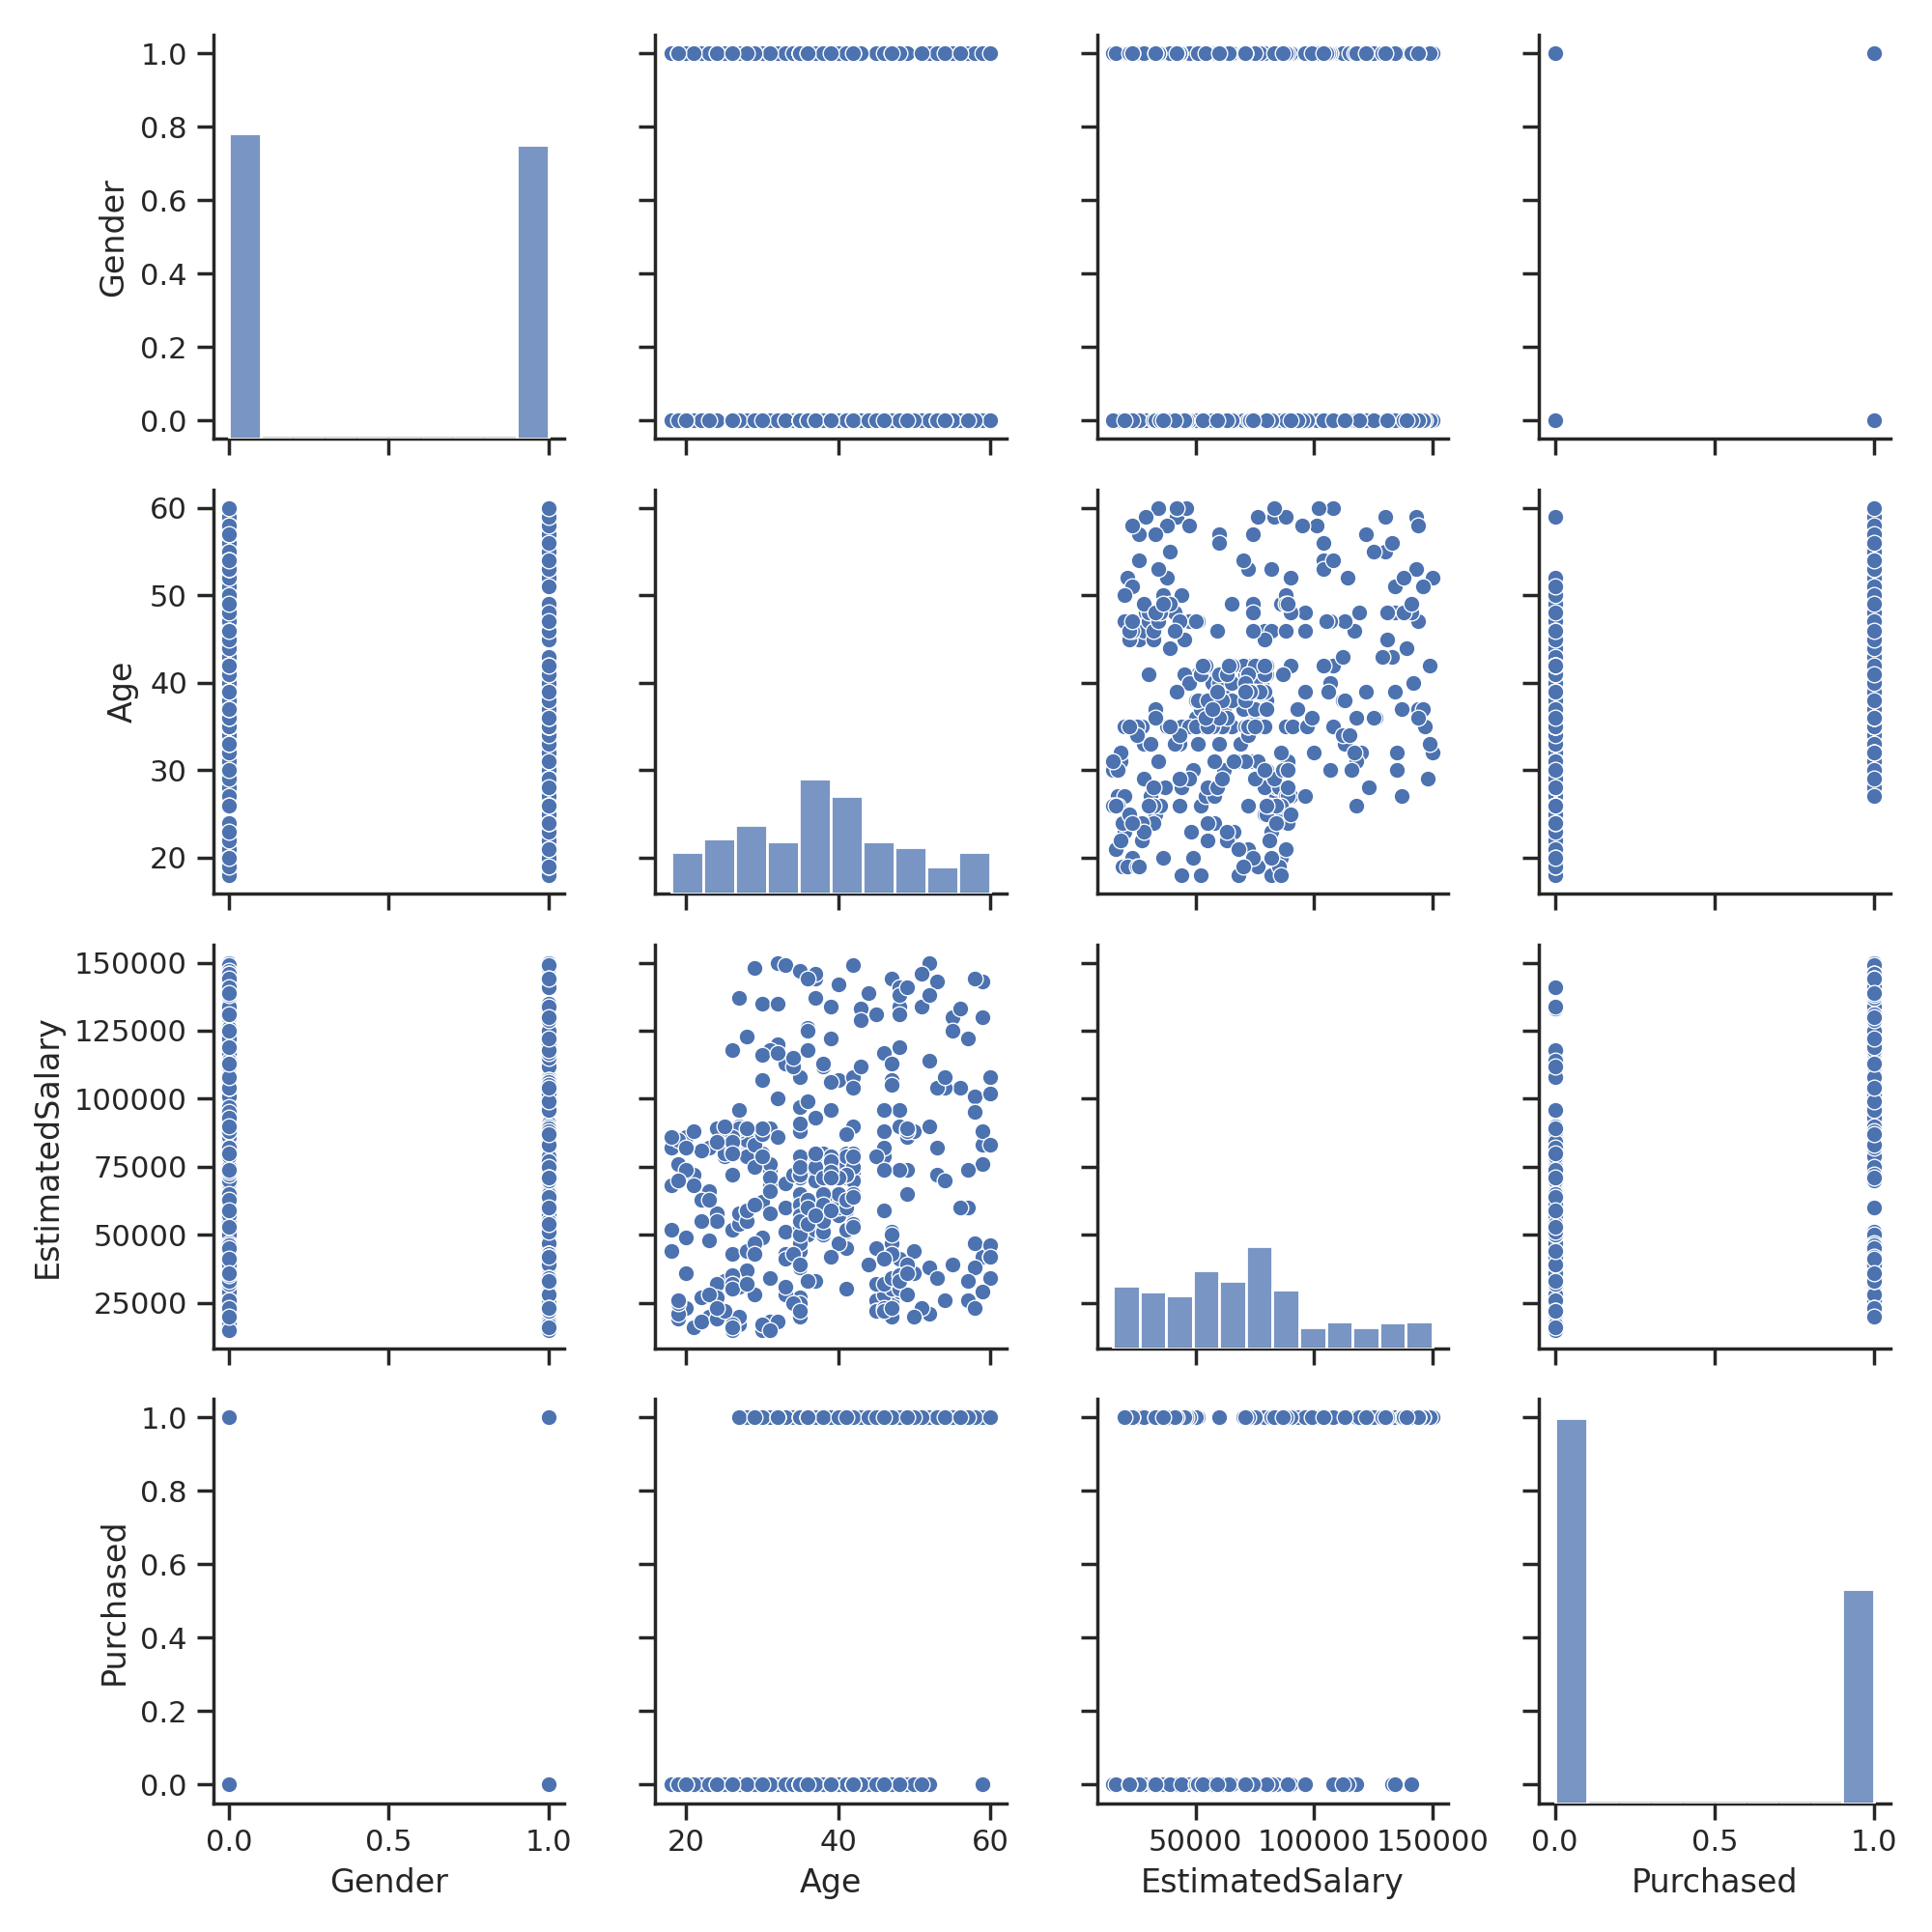
\includegraphics[width=0.8\textwidth]{../plots/social_pairplot_original.png}
	\caption{ Distributions and pair-wise correlation for the features of the "Titanic" data set.}
	\label{pairplot_income}
\end{figure}


\begin{figure}[h!]
	\centering
	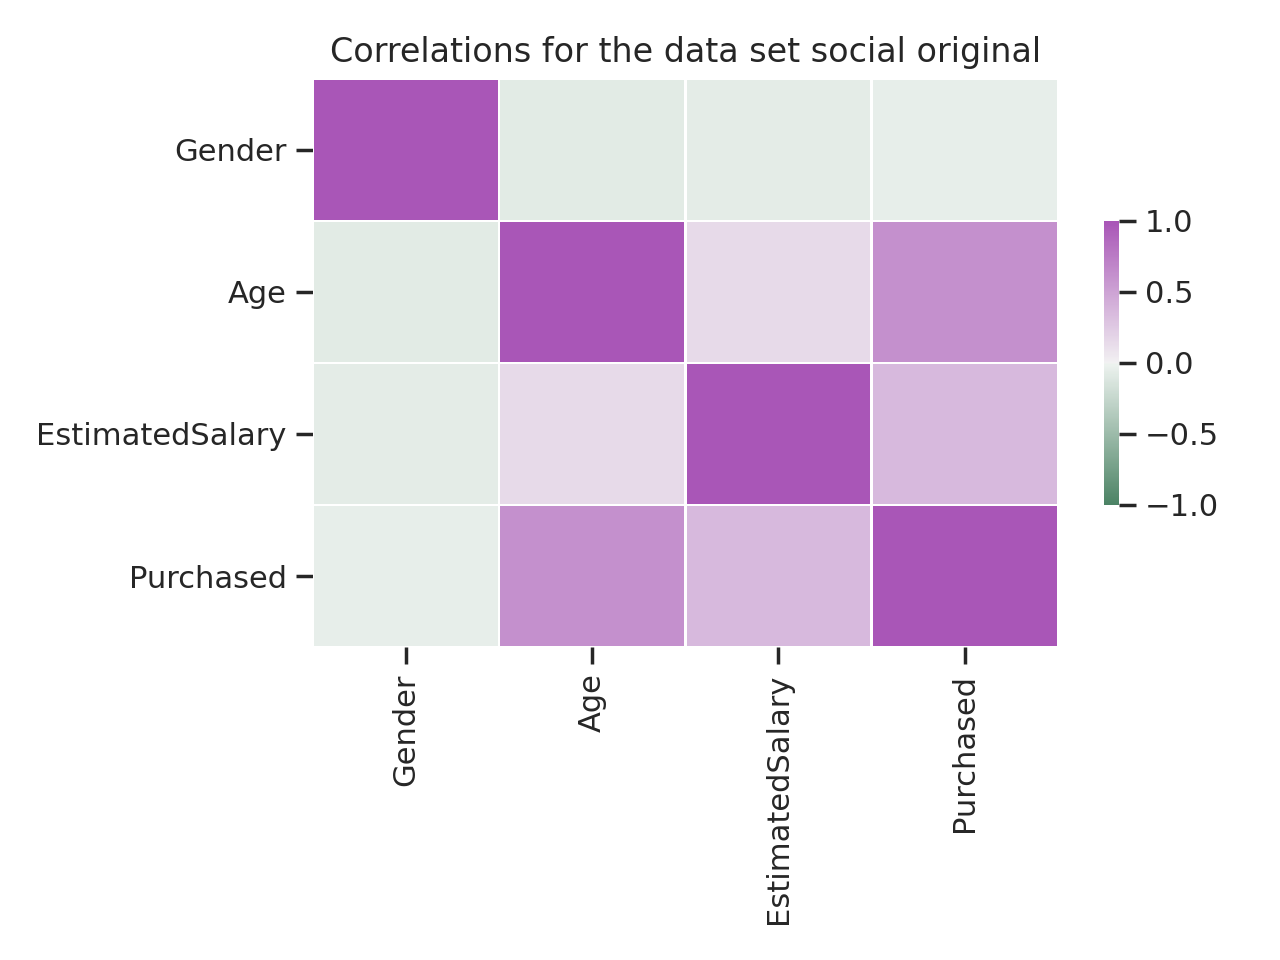
\includegraphics[width=0.5\textwidth]{../plots/social_correlations_original.png}
	\caption{Correlation matrix for the "Titanic" data set. }
	\label{correlation_income}
\end{figure}


\section{Workflow Overview and Code Structure}
Here we outline the structure of the code. The Project is build using the \textit{python3.8} language and various standard libraries such as \textit{pandas} and \textit{numpy} (for basic data import and analysis), \textit{sklearn} (sci-kit learn for model training and evaluation), \textit{} (for the creation of the synthetic data sets), \textit{matplotlib} and \textit{seaborn} for data visualization.

The project includes five different scripts that perform different tasks:

\begin{itemize}
	\item \textit{clean\_dataset.py}: module for the loading and cleaning of the input data sets. It reads the input data sets ad \textit{pandas} data frames, which are the main format handled by the library for model training. Among the cleaning of the data, we find the outlier removals and data rescaling;\

	\item  \textit{generate\_data.py}: module for the creating of synthetic data, based on the \textit{SDV} library;\


	\item  \textit{classifier.py}: main module of the project, contains the main functionalities to perform all the steps from data loading, cleaning, generation of synthetic data, model training and comparison of results;\

	\item \textit{utils.py}: module containing utilities e.g. for data plotting;\

\end{itemize}

In addition, a directory named "input\_data" is used to contain the input data sets as well as their respective cleaned version.
To run the entire project it is sufficient to first call the \textit{clean\_dataset.py} module e.g.
\begin{verbatim}
python3.8 clean_dataset.py
\end{verbatim}

This step will produce the cleaned data set inside the same "input\_data" directory as well as some control plots to show the distributions and correlation of the data.
\\


In the second step it is required to run with
\begin{verbatim}
python3.8 classifier.py
\end{verbatim}
that follows the following procedure:

\begin{enumerate}
	\item splitting of the original cleaned dataset into \textit{train} and \textit{test} sets, using a ratio of $70\%-30\%$ respectively; \

	\item  training and evaluation of the original dataset using the chosen classifier (random forest);


	\item  creation of the synthetic data sets, using the training set from the previous splitting of the original dataset, for the three models GaussianCopula,CTGAN and Copula GAN (see \ref{sec::synthetic});

	\item evaluate the models trained with the original and the synthetic dataset with the test set, obtained from the original model.

\end{enumerate}



\section{Data Exploration and Pre-processing}
In this section we describe the necessary preliminary steps to import and prepare the data to make them suitable for the learning algorithms.

The steps are handled by the script \textit{data\_preparation.py} which includes dedicated function to pre-process each data set.

\subsection{Data Overview}
Here we provide an overview of the original data.

\paragraph{Normalization}
Since we will be working with a random forest classifier, normalization is not needed for the data. Same goes for the SVD methods that should only fit distributions to the data and handle everything on their own.

\paragraph{Labelling}
In all datasets were present not numeric features. In order to synthetize them was necessary to change the strings into numeric values. In order to do so we used the cat.code method in this way for every not numeric features all the possible values where labelled using a different value. Using the labelling we had the possibility to use the three models.

\section{Generation of Synthetic Data} \label{sec::synthetic}
In order to generate the synthetic data we relied on three different generation models. The models are defined in the \textit{SDV} library. The three models aim to generate a synthetic data set whose properties are the same as in the original dataset. The three models we used are: GaussianCopula model, CTGAN model, CopulaGAN model.
We now describe the idea behind these three models as reported on the SDV library user guide.

\paragraph{GaussianCopula}
The Gaussian copula model \cite{gaussiancopula} is based on copulas which are distributions on [0;1]$^d$ which is constructed from a multivariate normal distribution over $\mathbb{R}^d$ by using the probability integral transform. Intuitively, a copula is a mathematical function that allows us to describe the joint distribution of multiple random variables by analyzing the dependencies between their marginal distributions.
\paragraph{CTGAN model}
The sdv.tabular.CTGAN model \cite{ctgan} is based on the GAN-based Deep Learning data synthesizer which was presented at the NeurIPS 2020 conference by the paper titled "Modeling Tabular data using Conditional GAN".
\paragraph{Copula GAN}
The sdv.tabular.CopulaGAN model \cite{copulagan} is a variation of the CTGAN Model which takes advantage of the CDF based transformation that the GaussianCopulas apply to make the underlying CTGAN model task of learning the data easier.



\section{Model Implementation and Evaluation}

We follow the schematic in Fig. \ref{fig:schematic}. Thus, splitting the original data set in a train- and test-set (70\% train data and 30\% test data), synthesizing new data according to the chosen syntheziser methods and traning a classifier on the new and original data set to compare them in a classification task, tested on the test-set.

\begin{figure}[h!]
	\centering
	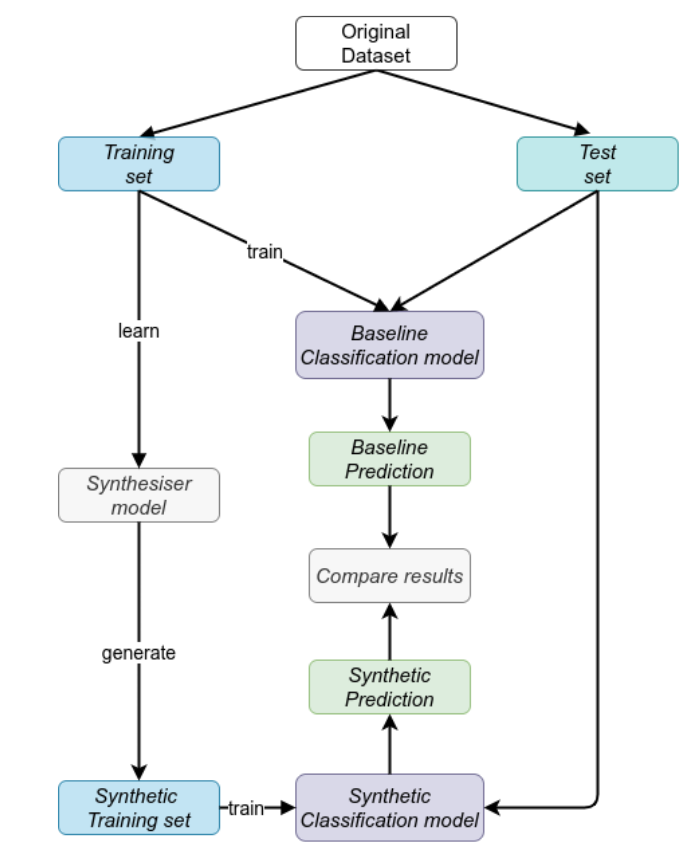
\includegraphics[width=0.45\textwidth]{pics/schematic.png}

	\caption{Outline of the used workflow.}
	\label{fig:schematic}
\end{figure}


\subsection{Classification}

The classification is done with a random forest classifier in a hold-out-validation fashion (using the previously created test-set). Since classification was already done in Exercise 1, we wont go in any further detail on the implementation. \\

To train our model, we used the \textit{schi-kit learn} implementation of a random forest algorithm \textit{RandomForestClassifier()} with default parameters.

\paragraph{Metrics}

We use accuracy, precision and, as a combination, the f1-score as a metric for the classification results. Since our task is the creation of data that is close to the original one with respect to the underlying structure, it is not majorly important to achieve good classification results, but to achieve similar results for the original and synthesized data set. Thus, we were not optimizing the classification. \\

Additionally as an optical metric, we use the confusion matrix to see the results of the classification. In a confusion matrix it is easy to see how well the classification performed by looking at the entries on the main diagonal - off-diagonal entries represent misclassifications. Again, the performance is not important but rather the similarity between the data sets.

\subsection{Confusion Matrices}
As outlined in the previous section, we classified both the original and synthetic data set and create the corresponding confusion matrices. Each entry $i,j$ corresponds to the number of observations in group $i$, but predicted to be in group $j$. We normalize the entries according to the sum of each row. Since it is a binary classification, the matrix reduces to the number of true negatives ($TN$), false positives ($FP$), false negatives ($FN$) and true positives ($TP$). We then analyzed the performance of the implementation using   precision ($P$) and recall ($R$), defined as :

\begin{equation}
P = \frac{TP}{TP + FP} \ \ \ \ \ \ \ \  R = \frac{TP}{TP + FN} \ \ \ \ \ \ \ \  A = \frac{TP + TN}{all}
\end{equation}

In this section we present the results of the confusion matrices, obtained after training our random forest classifier on the original data set and on the three different synthetic data sets. Results for the titanic, income and social data sets are shown respectively in Figures \ref{confusion_titanic}, \ref{confusion_income} and \ref{confusion_social}.


\begin{figure}[h!]
	\centering
	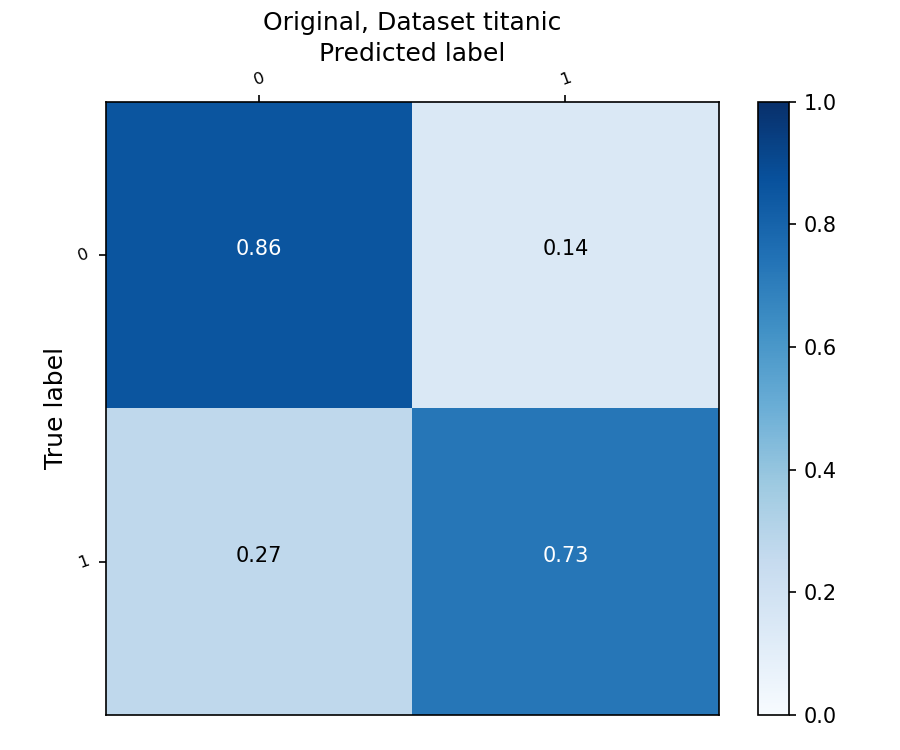
\includegraphics[width=0.45\textwidth]{../ConfusionMatrixes/titanic_Original_.png}
	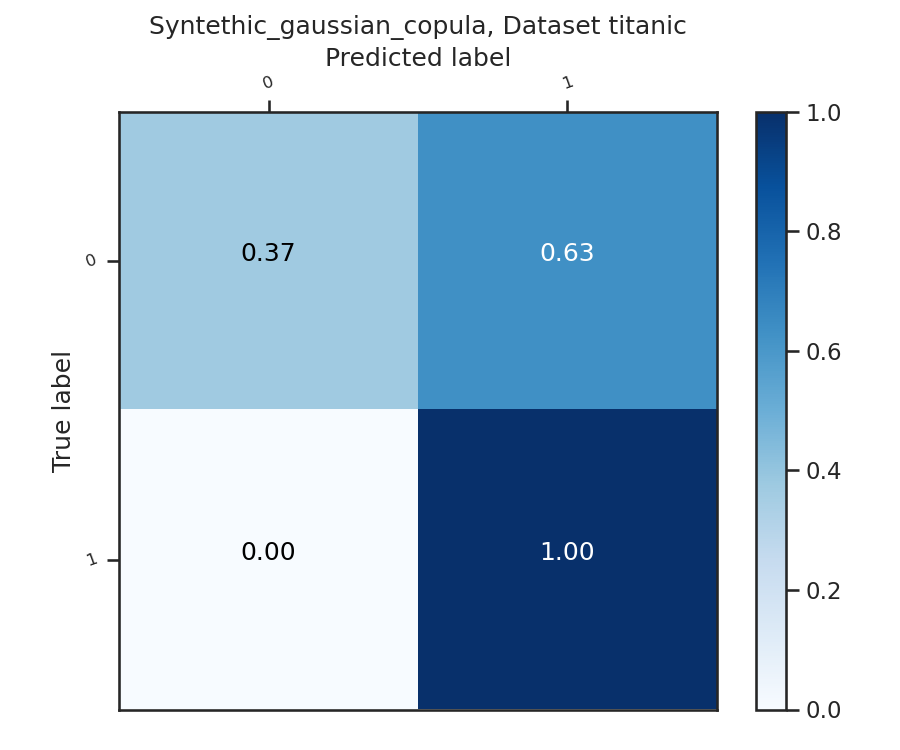
\includegraphics[width=0.45\textwidth]{../ConfusionMatrixes/titanic_Syntethic_gaussian_copula_.png}
	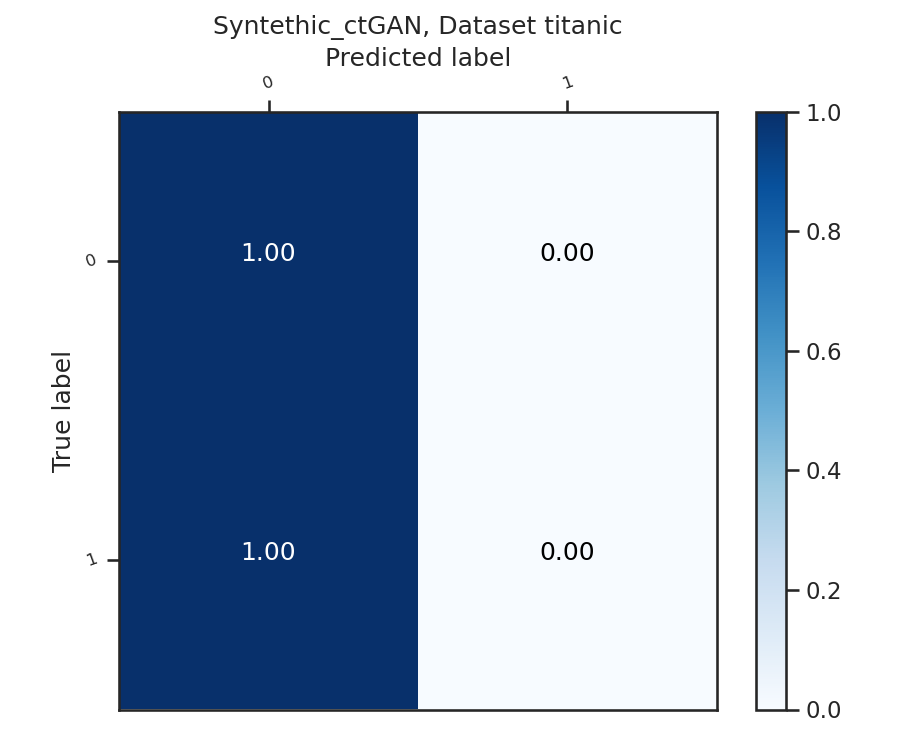
\includegraphics[width=0.45\textwidth]{../ConfusionMatrixes/titanic_Syntethic_ctGAN_.png}
	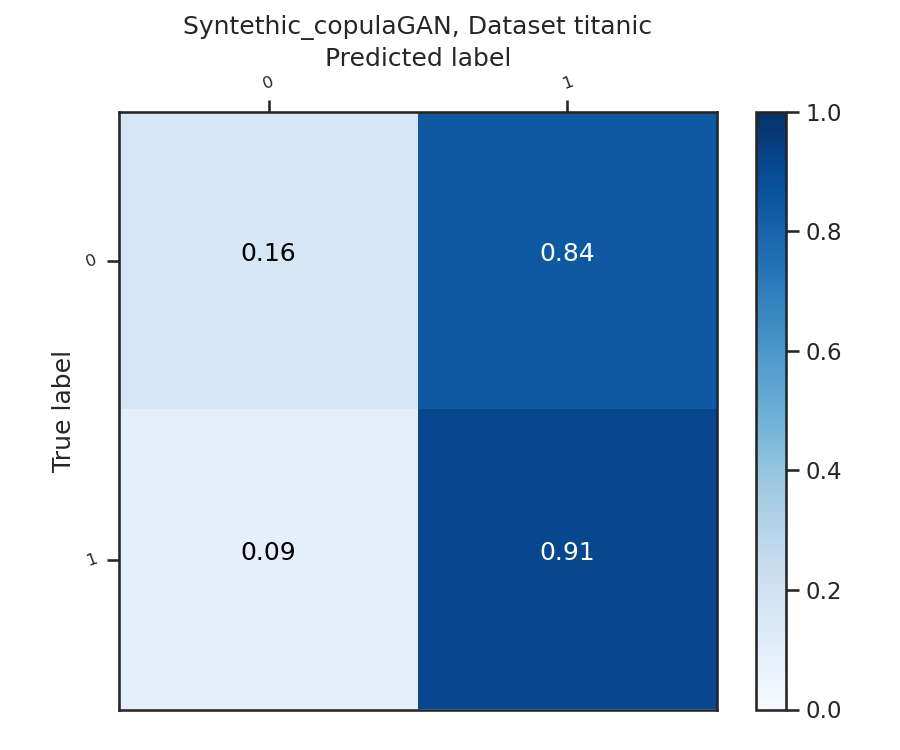
\includegraphics[width=0.45\textwidth]{../ConfusionMatrixes/titanic_Syntethic_copulaGAN_.png}

	\caption{Confusion matrices for the "Titanic" data set: original dataset (top-left panel), Gaussian Copula synthetic data set (top-right panel), GAN synthetic data set (bottom-left panel) and GAN Copula synthetic data set (bottom-right panel).  }
	\label{confusion_titanic}
\end{figure}

\begin{figure}[h!]
	\centering
	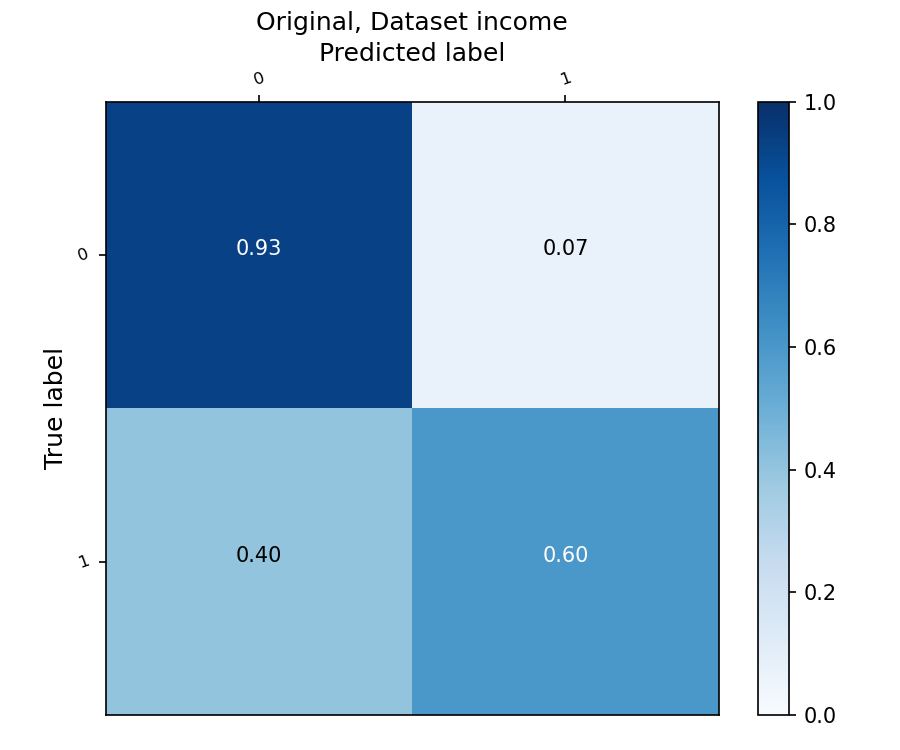
\includegraphics[width=0.45\textwidth]{../ConfusionMatrixes/income_Original_.png}
	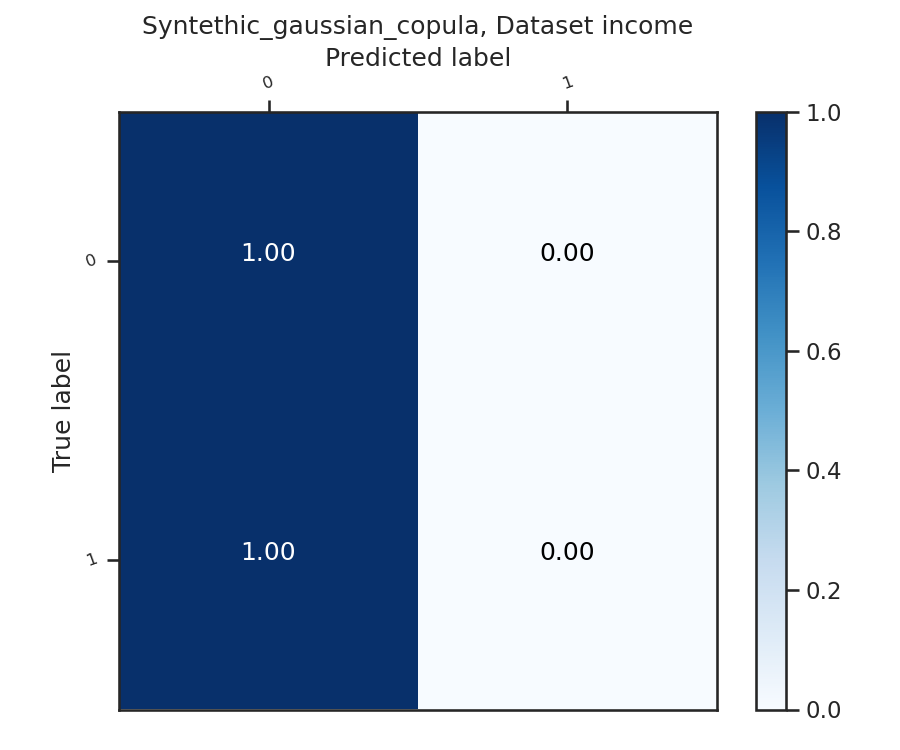
\includegraphics[width=0.45\textwidth]{../ConfusionMatrixes/income_Syntethic_gaussian_copula_.png}
	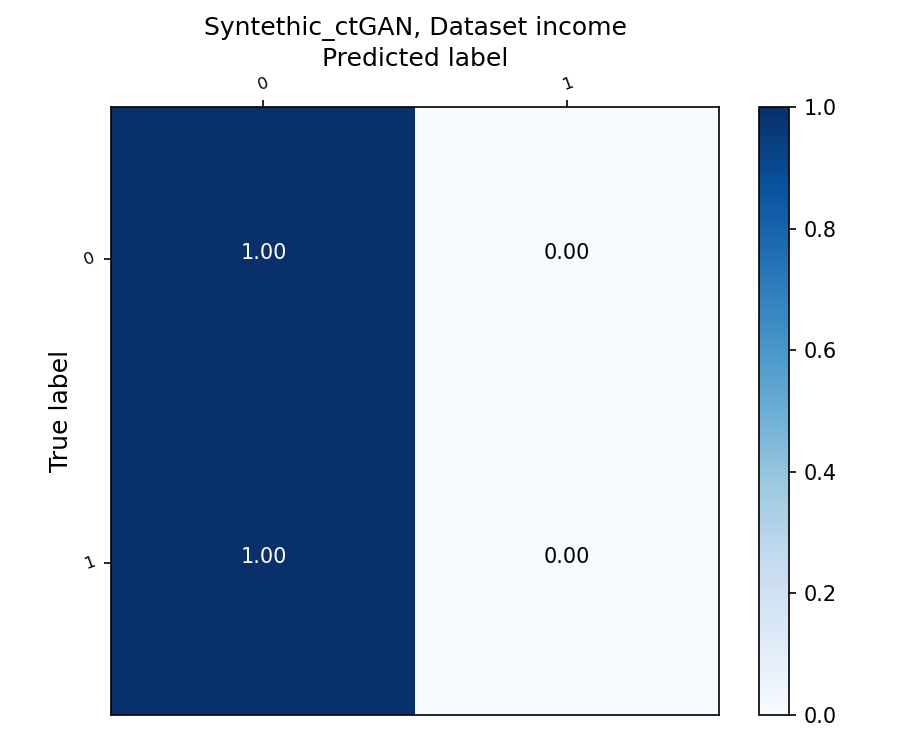
\includegraphics[width=0.45\textwidth]{../ConfusionMatrixes/income_Syntethic_ctGAN_.png}
	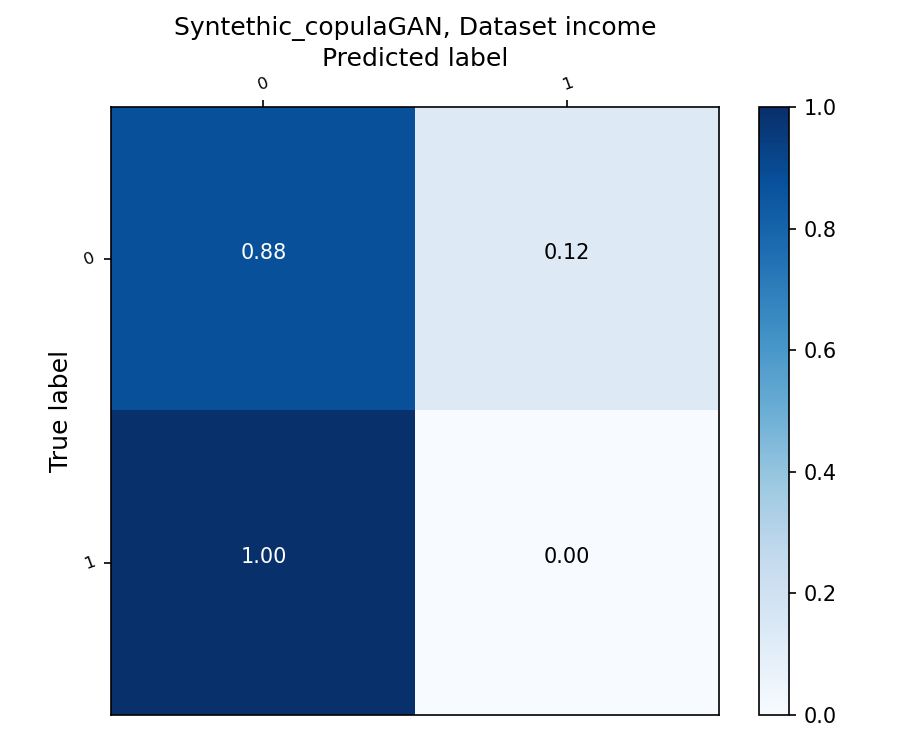
\includegraphics[width=0.45\textwidth]{../ConfusionMatrixes/income_Syntethic_copulaGAN_.png}

	\caption{Confusion matrices for the "Income" data set: original dataset (top-left panel), Gaussian Copula synthetic data set (top-right panel), GAN synthetic data set (bottom-left panel) and GAN Copula synthetic data set (bottom-right panel).  }
	\label{confusion_income}
\end{figure}


\begin{figure}[h!]
	\centering
	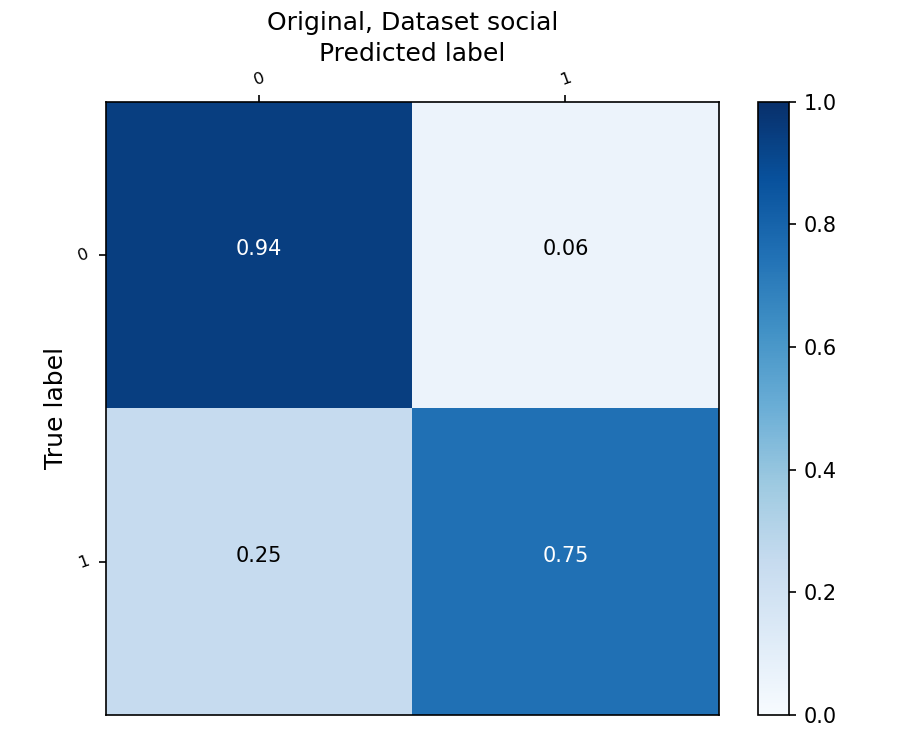
\includegraphics[width=0.45\textwidth]{../ConfusionMatrixes/social_Original_.png}
	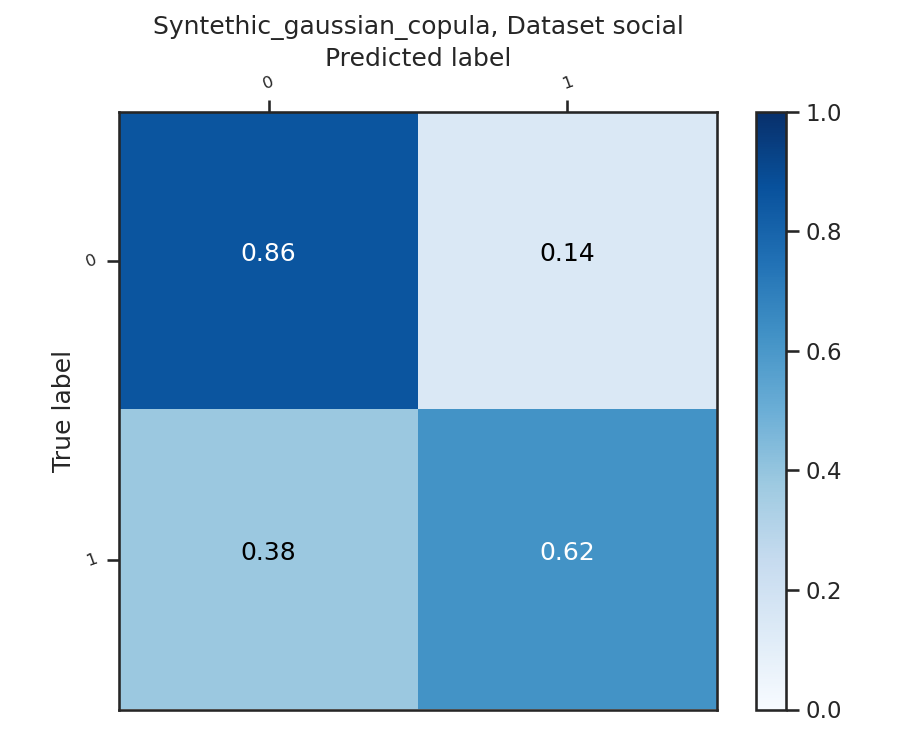
\includegraphics[width=0.45\textwidth]{../ConfusionMatrixes/social_Syntethic_gaussian_copula_.png}
	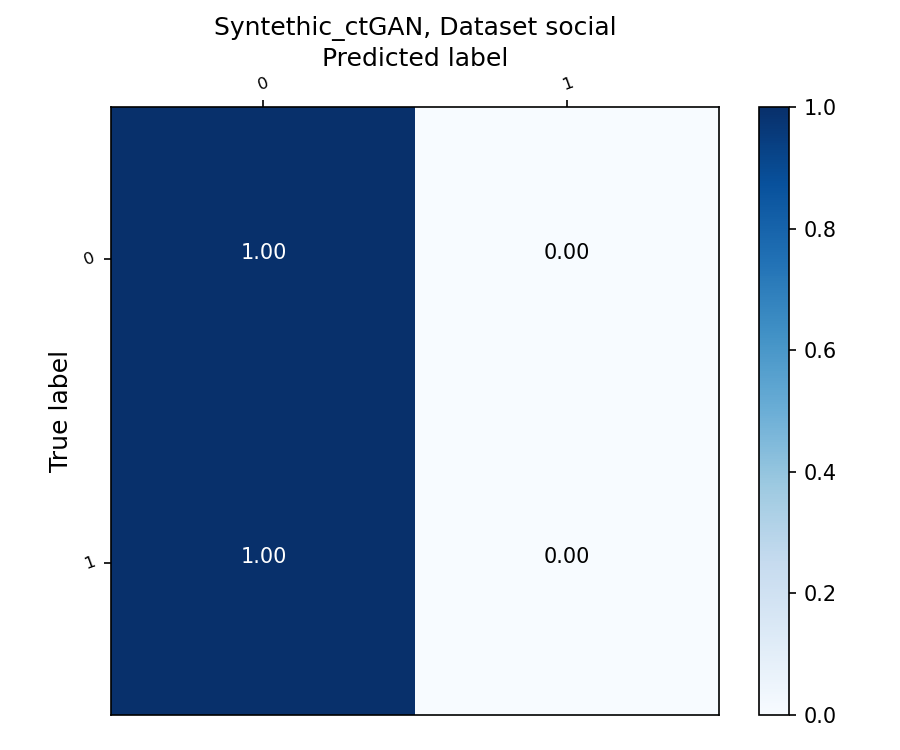
\includegraphics[width=0.45\textwidth]{../ConfusionMatrixes/social_Syntethic_ctGAN_.png}
	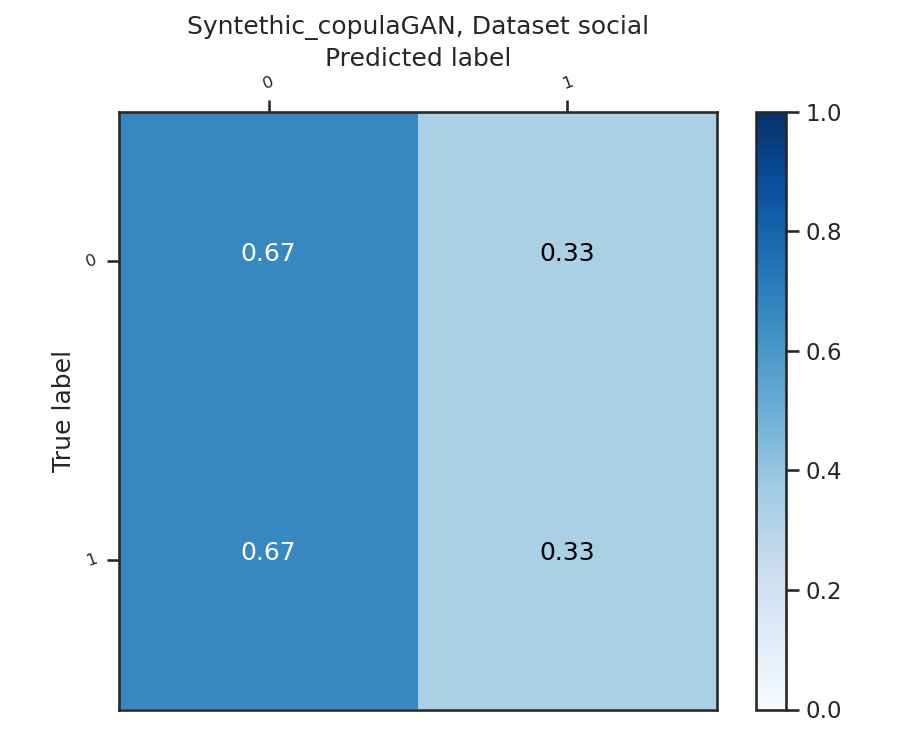
\includegraphics[width=0.45\textwidth]{../ConfusionMatrixes/social_Syntethic_copulaGAN_.png}

	\caption{Confusion matrices for the "Social" data set: original dataset (top-left panel), Gaussian Copula synthetic data set (top-right panel), GAN synthetic data set (bottom-left panel) and GAN Copula synthetic data set (bottom-right panel).  }
	\label{confusion_social}
\end{figure}

\subsection{Scores}
Finally, in Figures \ref{scores_titanic} , \ref{scores_income} and \ref{scores_social} we show the values for the precision, accuracy and recall obtained after training the random classifier on the 4 different input data sets (original and three synthetic ones).


\begin{figure}[h!]
	\centering
	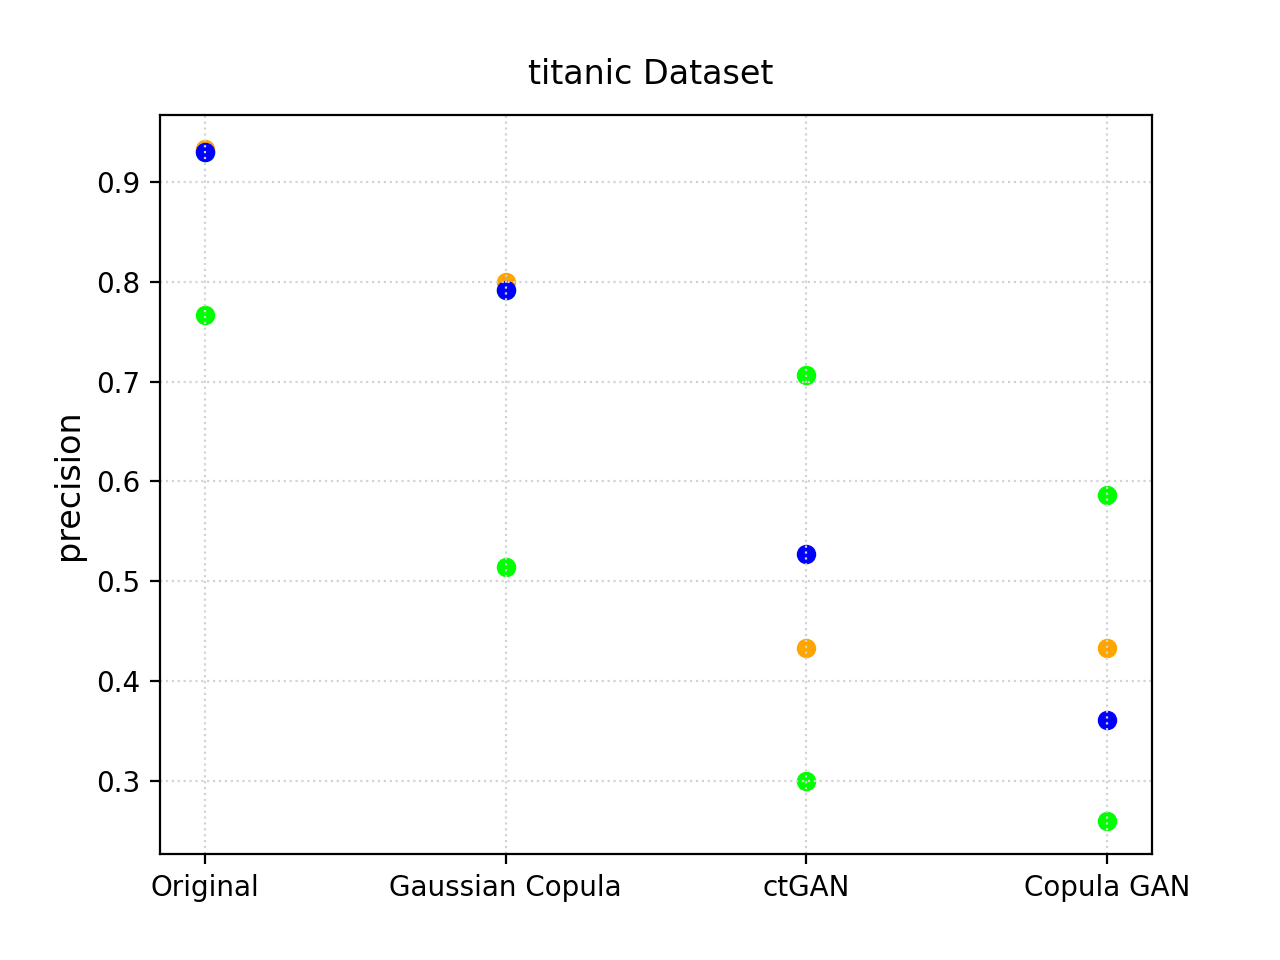
\includegraphics[width=0.32\textwidth]{../plots/results/titanic_precision.png}
	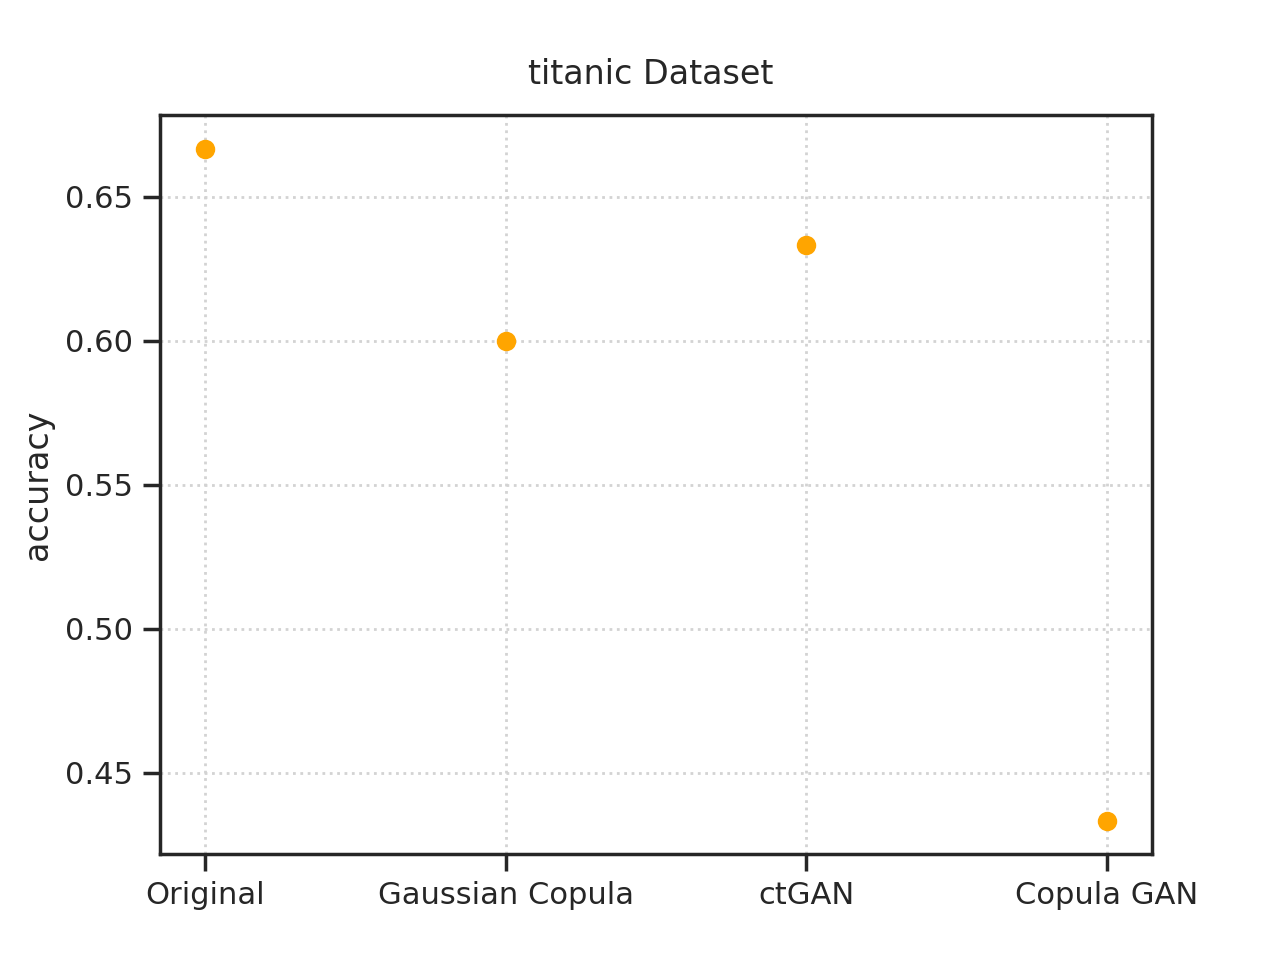
\includegraphics[width=0.32\textwidth]{../plots/results/titanic_accuracy.png}
	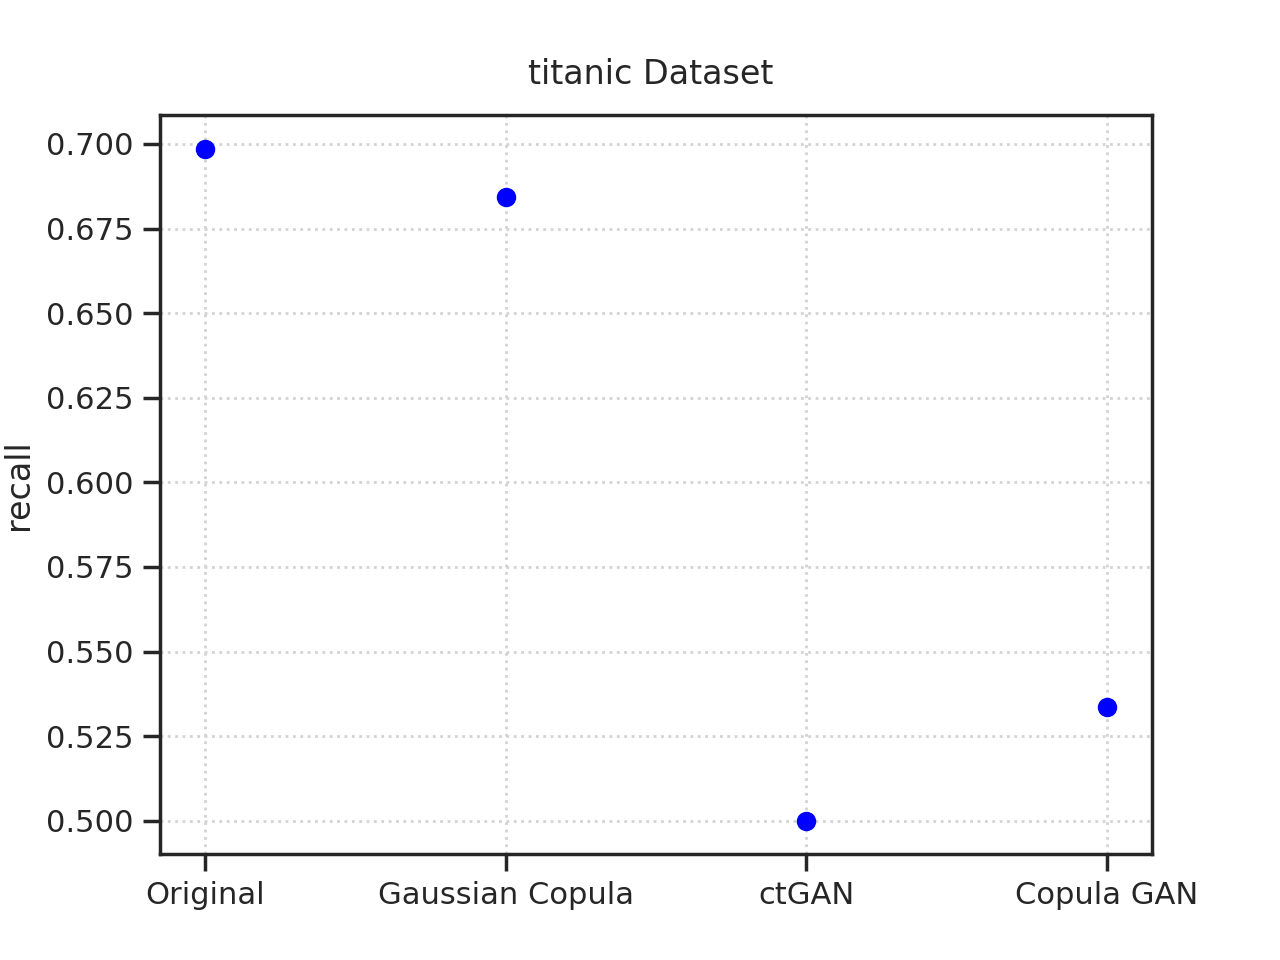
\includegraphics[width=0.32\textwidth]{../plots/results/titanic_recall.png}

	\caption{Precision, accuracy and recall scores for the rand forest classifier, trained on the original data set and on the three synthetic data sets, for the "Titanic" data set.}
	\label{scores_titanic}
\end{figure}


\begin{figure}[h!]
	\centering
	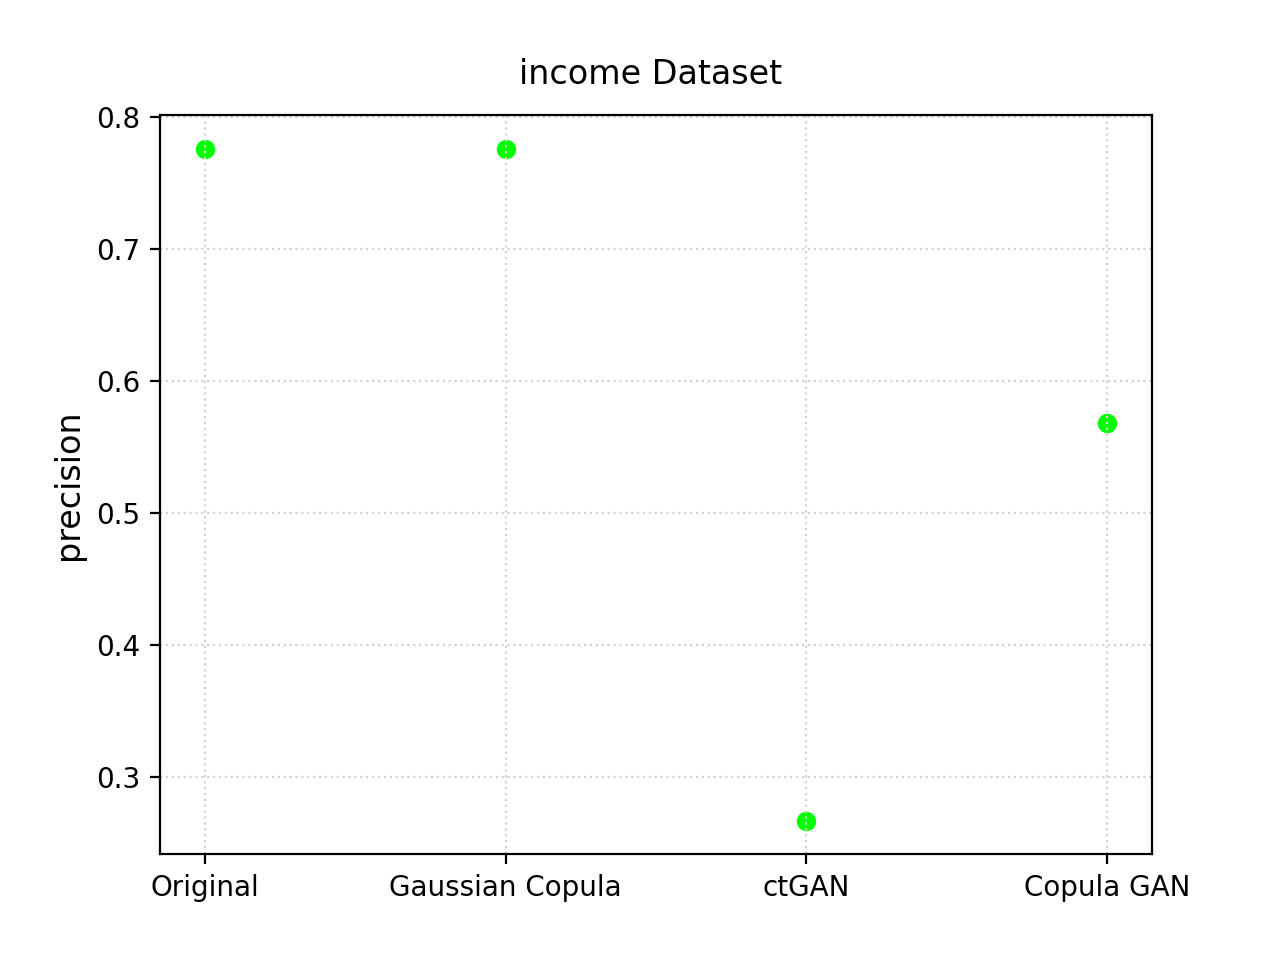
\includegraphics[width=0.32\textwidth]{../plots/results/income_precision.png}
	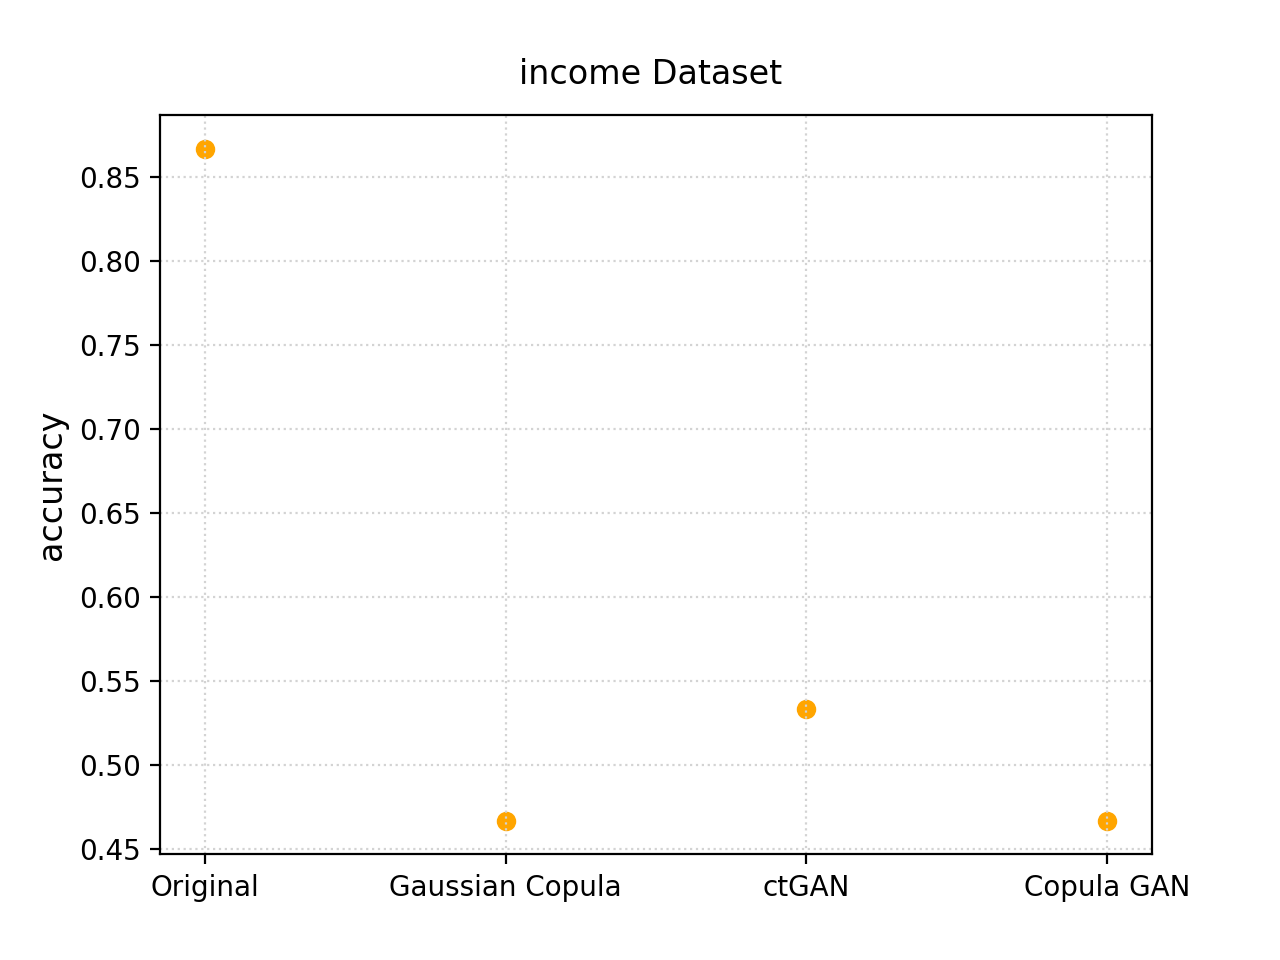
\includegraphics[width=0.32\textwidth]{../plots/results/income_accuracy.png}
	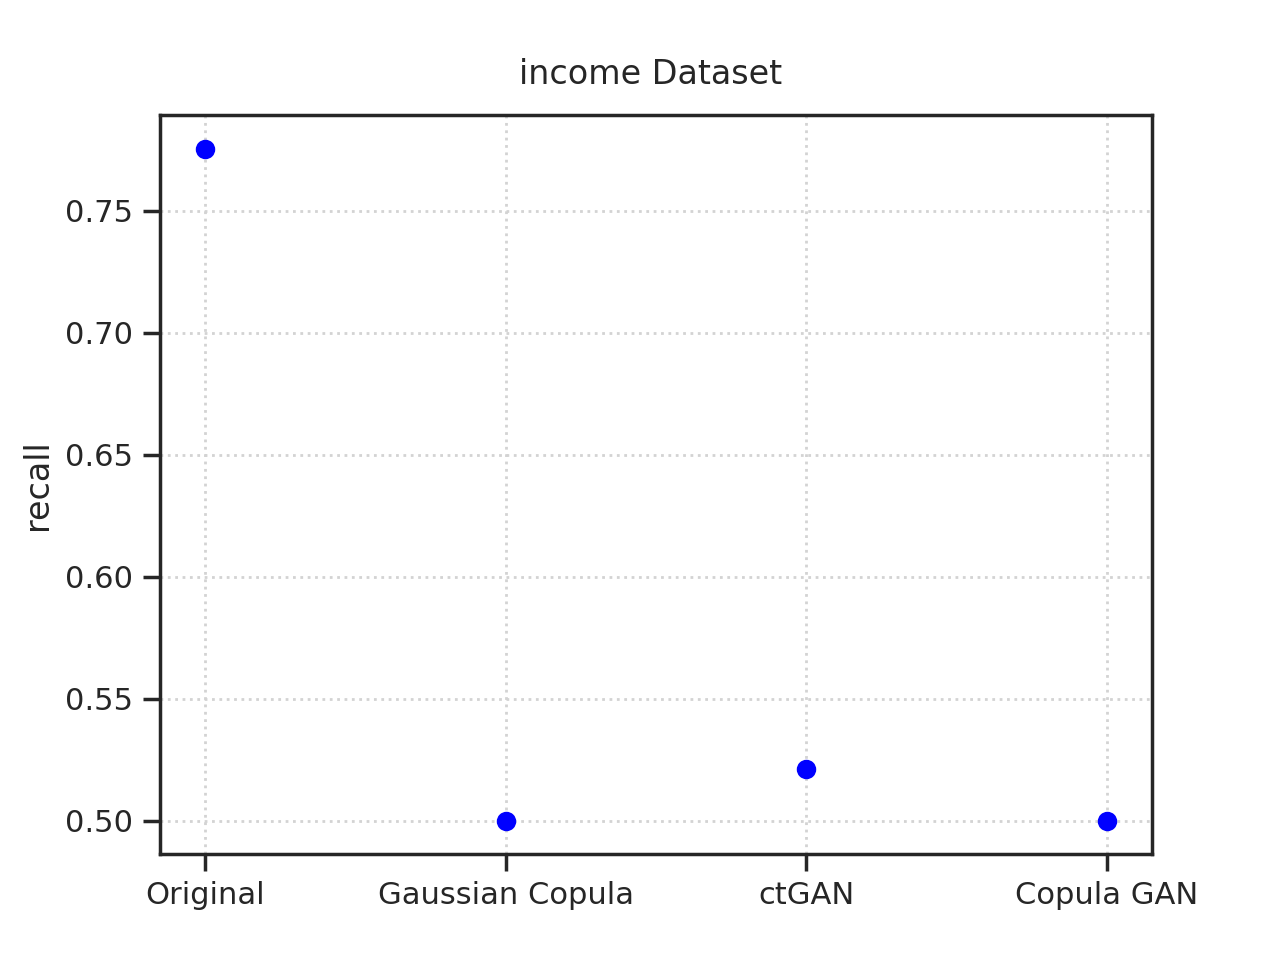
\includegraphics[width=0.32\textwidth]{../plots/results/income_recall.png}

	\caption{Precision, accuracy and recall scores for the rand forest classifier, trained on the original data set and on the three synthetic data sets, for the "Titanic" data set.}
	\label{scores_income}
\end{figure}

\begin{figure}[h!]
	\centering
	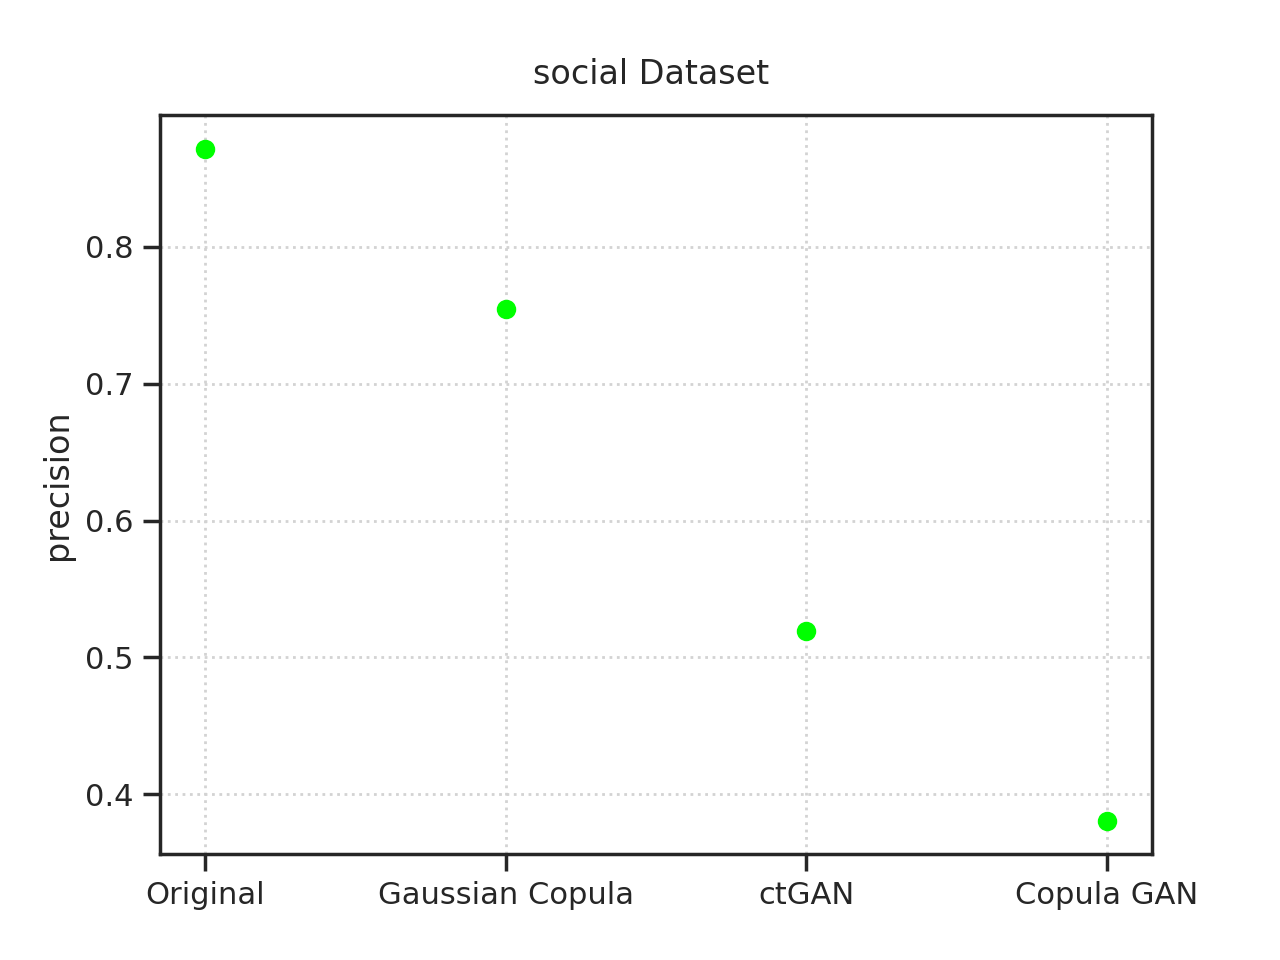
\includegraphics[width=0.32\textwidth]{../plots/results/social_precision.png}
	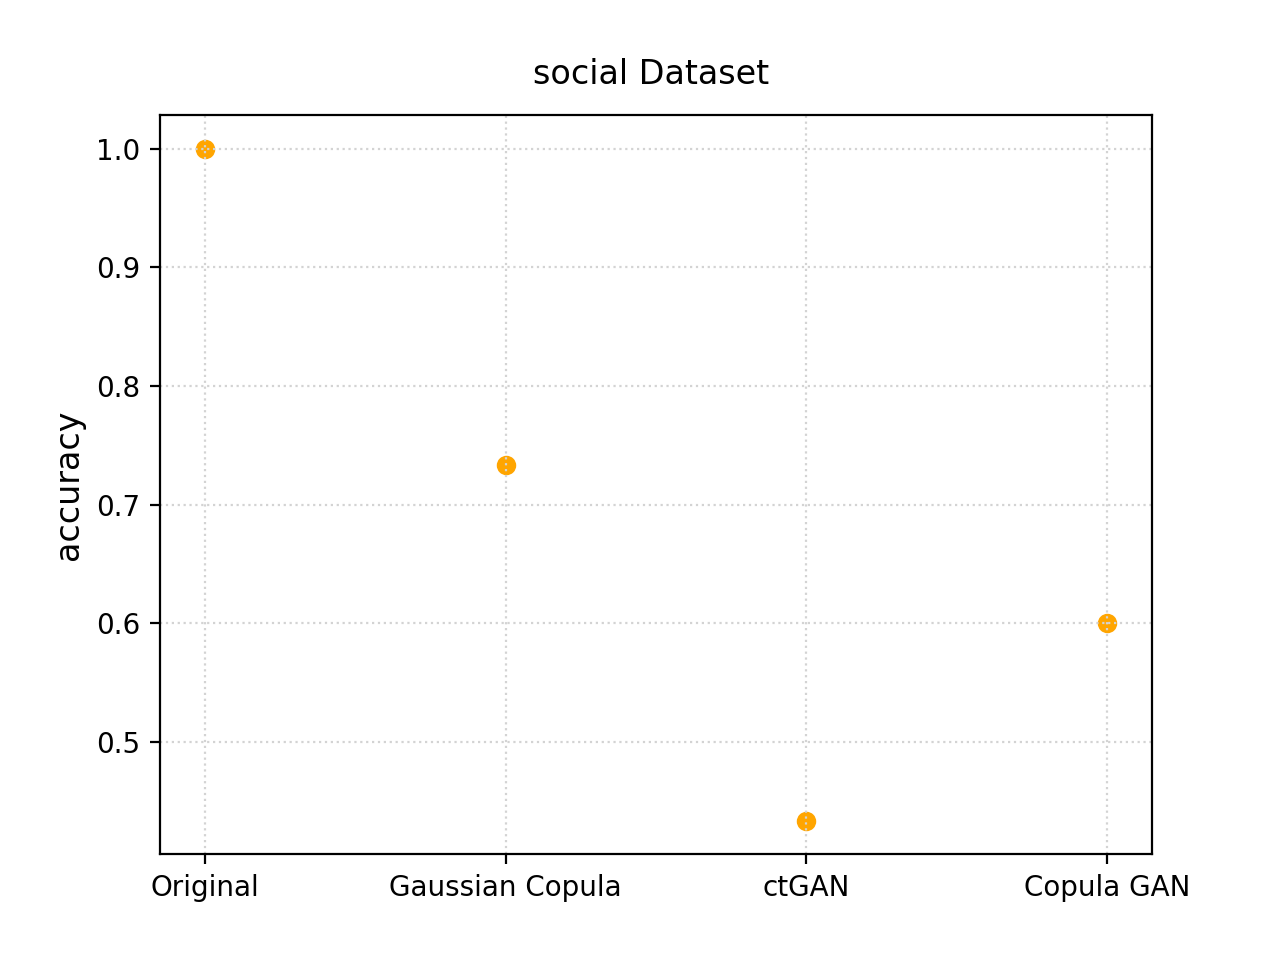
\includegraphics[width=0.32\textwidth]{../plots/results/social_accuracy.png}
	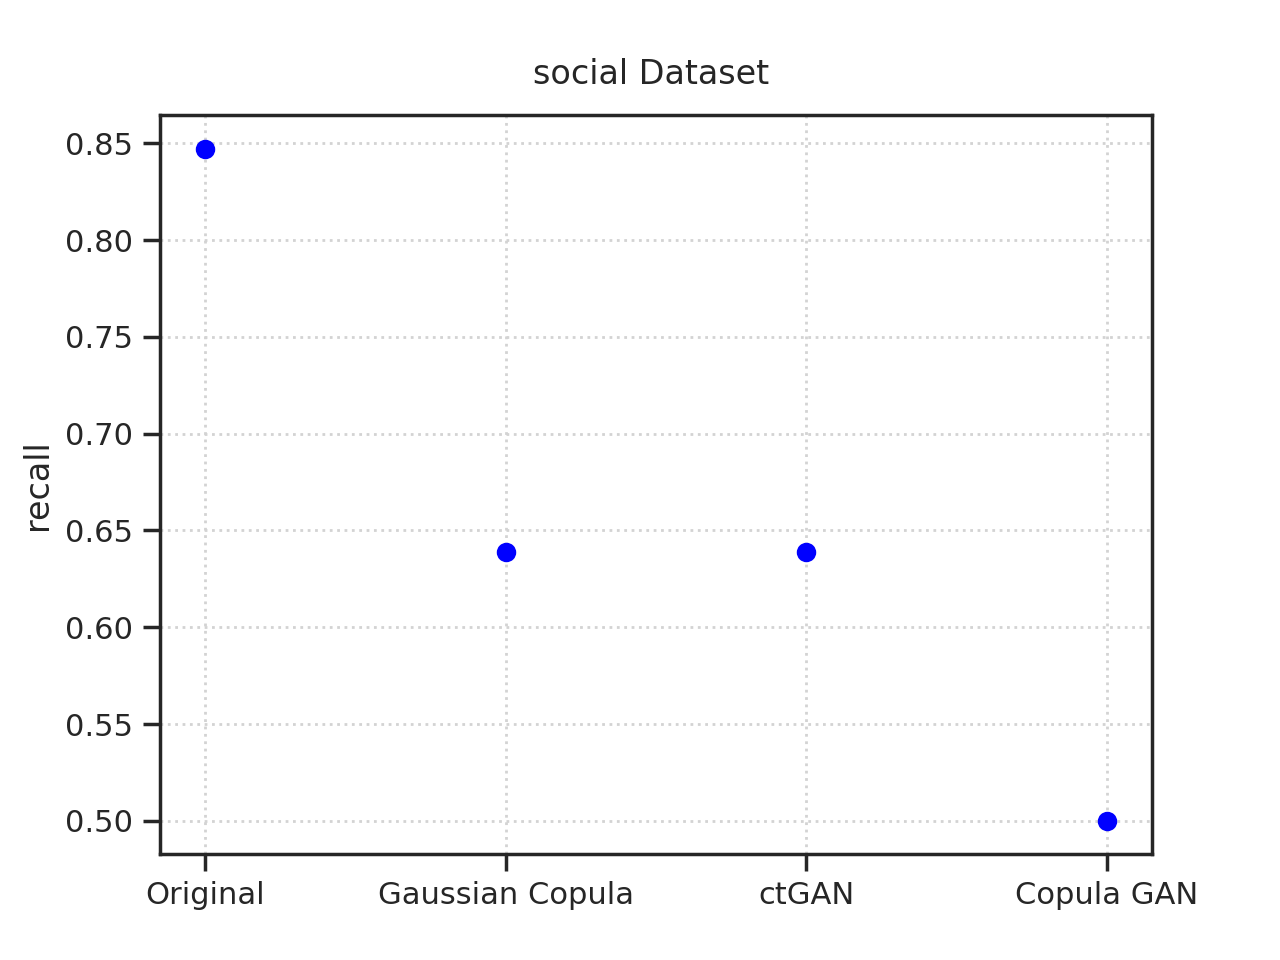
\includegraphics[width=0.32\textwidth]{../plots/results/social_recall.png}

	\caption{Precision, accuracy and recall scores for the rand forest classifier, trained on the original data set and on the three synthetic data sets, for the "Social" data set.}
	\label{scores_social}
\end{figure}




\clearpage
\section{Conclusion}

As can be seen in the figures above, the outcome of the data synthesizing depends on the underlying data set and the used SDV method. On the "adult income" dataset all methods produce a data set for which the best strategy of the Random Forest (RF) classifier is to constantly guess the same class. This makes sense when looking at the produced data - mainly data points of one class are produced. We did not find out what could be the cause for this and could be further investigated. But since the documentation on the SDV methods is rather sparse and it is not point of this assignment we will skip this. \\

For the other two data sets the \textit{GaussianCopula} method was performing the best out of the SDV methods and actually gives quite reasonable results. \textit{ctGAN} gives a low performance on all data sets and the RF classifier returns a trivial strategy (same reasons as before). The result for \textit{copulaGAN} is rather surprising. Having lots of entries off the main diagonal, the synthesizer seems to often swap (binary labels) the labels a data point would normally have - he does this consistently with both classes. \\

Looking at the metrics we can see, again, that the \textit{GaussianCopula} is performing the best out of our synthesizers. But looking at those metrics one could assume that \textit{ctGAN} performs halfway between \textit{GaussianCopula} and \textit{copulaGAN}. This is of course a deception since both are performing bad, only that \textit{ctGAN} makes correct guesses for one of the classes. \\

We cannot see what in the "adult income" data set causes it to perform so bad. It has a similar amount of features to the "titanic" data set and has a mixture of categorical and non-categorical features. It is a bit heavy on the categorical features though - testing it on a subset of the features could be a way to test for improvement. It is also by far the biggest data set having 32.560 entries (compared to 891 in the "titanic" and 400 in the "social media ad" data sets). But we don't see how more data could negatively affect the results of the synthesizer methods. \\

To wrap everything up, we think that the lack of a deep understanding on the production of the synthetic data, was limiting our ability to easily improve the results. We would've had the best shot by simply trying out a lot of things to hope and find an underlying pattern in the response of the model. 

\clearpage
\bibliography{literature.bib}{}
\bibliographystyle{unsrt}

\end{document}
